\documentclass[11pt,a4paper]{article}
\usepackage{fontspec}
\setmainfont{Source Serif 4}[Path=/home/claude/ref/fonts/, UprightFont=SourceSerif4-Regular.ttf, BoldFont=SourceSerif4-Semibold.ttf, ItalicFont=SourceSerif4-It.ttf]
\setmonofont{IBM Plex Mono}[Path=/home/claude/ref/fonts/, UprightFont=IBMPlexMono-Regular.ttf, BoldFont=IBMPlexMono-Medium.ttf, Scale=0.88]
\usepackage[margin=2.5cm]{geometry}
\usepackage{graphicx,booktabs,longtable,array,caption,amsmath,xcolor,setspace,threeparttable}
\usepackage[authoryear,round]{natbib}
\usepackage[hidelinks]{hyperref}
\usepackage{microtype}
\setstretch{1.12}
\captionsetup{font=small,labelfont=bf}
\setlength{\bibsep}{3pt}
\title{\textbf{Does Parliament Notice Disasters, and Whose? Attention in the House of Commons to the Places of UK Disasters, 1910 to 2020}}
\author{Dr Tristan Hotham\\\small Independent researcher\\\small ORCID 0000-0003-4931-9349}
\date{2026}
\begin{document}
\maketitle
\begin{center}\textbf{Abstract}\end{center}
Disasters are classic focusing events, but how much attention do legislatures give the places where they happen? I link 64 localised UK disasters, 1910 to 2020, to monthly counts of House of Commons contributions naming the place. In a stacked Poisson event study pre-specified in a written plan, attention rises to 10.4 times its pre-event level in the month of the disaster (95\% CI 2.4 to 44.9); the median disaster accrues half its five-year excess within 8.5 months, though some followed by inquiries hold attention for years. Five-year attention rises with deaths far less than proportionally (elasticity 0.42, CI 0.05 to 0.78), but the interval includes zero in 12 of 28 planned checks. Adding 22 disasters that became searchable later gives 0.52 (CI 0.12 to 0.92), still fragile. A London and South East premium rests on two events. Lists of remembered disasters and search phrases shape these results.

\medskip\noindent\textbf{Keywords:} focusing events; agenda setting; issue-attention cycle; disasters; House of Commons; Hansard; political attention; United Kingdom

\section{Introduction}
\label{sec:intro}
When a mine explodes, a stadium crush kills supporters or a tower block burns, the name of the place often becomes part of the national vocabulary: Aberfan, Hillsborough, Lockerbie, Grenfell. Students of public policy have long treated such events as \emph{focusing events}: sudden, rare and harmful occurrences that concentrate the attention of the public and of policy makers on a problem \citep{Kingdon1984,Birkland1997,Birkland1998}. The agenda-setting tradition argues that attention is scarce and that its allocation shapes what governments do \citep{BaumgartnerJones1993,JonesBaumgartner2005}. The issue-attention cycle predicts that interest in a problem rises sharply and then fades, often before anything is resolved \citep{Downs1972}. Disaster research adds that the political response is contested: who is blamed, what lessons are drawn and whether anything changes depend on framing contests, on the persistence of the bereaved and on the institutions that investigate \citep{Boin2005,Boin2009,Hood2011,Birkland2006}.

Despite this, there is little systematic evidence on the most basic quantity: how much attention does a national legislature give to the place of a disaster, for how long, and does that attention follow the scale of the loss or the location of the people who died? Work on media and government responses to disasters in the United States and elsewhere suggests that attention depends on competing news and on who the victims are \citep{EisenseeStromberg2007,Stromberg2007}, and that political rewards follow relief more than preparedness \citep{HealyMalhotra2009,GarrettSobel2003}. British studies of individual disasters, such as Aberfan and Hillsborough, describe long struggles for recognition and accountability \citep{McLeanJohnes2000,Johnes2000,Scraton1999}, and press coverage of British man-made disasters has been studied as a site of anger and citizenship \citep{PanttiWahlJorgensen2011}. But no study has followed a large set of UK disasters through the parliamentary record with a common measure.

This paper does that. I build a curated list of 64 localised disasters in the UK from 1910 to 2020, from mining explosions and rail crashes to bombings and fires, and count, month by month, the House of Commons contributions that name the place, using the UK Parliament's Hansard search \citep{Hansard2026}. Three questions guide the analysis. First, how large is the rise in attention and how fast does it fade? Second, does attention scale with the death toll? Third, does it depend on where the disaster happened: in London and the South East or elsewhere, in England or in Scotland, Wales and Northern Ireland, and in mining communities?

The analysis plan, including the inclusion rules, the measures, the models, the robustness checks and what would count against each hypothesis, was written down before any outcome model was run, and the planned specifications are reported as the main results. Two departures are documented: a clarification of the rule for choosing search terms and the exclusion of one event under the plan's own rule, both made before any model was estimated. Analyses added after the planned results were seen are labelled as exploratory. A third departure came later: once the search phrases that the first version lacked had been harvested, I added the events they made searchable under the same rules. That extension was made after the first results were known, so it is reported beside the first version (Section~\ref{sec:ext}), not in place of it.

The findings are, in brief, as follows. Commons attention to the place rises sharply, to about 10 times its usual level in the month of the disaster, and most of the excess comes early: half of the five-year excess is reached in a median of 8.5 months. A small number of disasters, usually those followed by public inquiries or long campaigns, sustain attention for years. Attention rises with the death toll, but much less than proportionally, and the association is fragile. Adding the 22 disasters that became searchable later strengthens the association (elasticity 0.52; permutation $p$ = 0.006), but it remains sensitive to specification. London and the South East appear to receive more attention for the same toll, but that difference rests on two events. There is no clear evidence of a deficit or premium for the devolved nations or for mining disasters. The paper also shows how strongly the list of disasters that is available to study, and the words used to search for them, shape what can be learned: both are filters of collective memory.

Section~\ref{sec:lit} reviews the literature. Section~\ref{sec:data} describes the data and the construction of the event list. Section~\ref{sec:design} sets out the design and hypotheses. Section~\ref{sec:results} presents the results, Section~\ref{sec:robust} the robustness checks and Section~\ref{sec:ext} the extended event list. Section~\ref{sec:discussion} discusses the findings and their limits, and Section~\ref{sec:conclusion} concludes.

\section{Background and literature}
\label{sec:lit}
\subsection{Focusing events and the scarcity of attention}
Kingdon's account of agenda setting describes problems that reach the governmental agenda through indicators, feedback and focusing events such as crises and disasters \citep{Kingdon1984}. \citet{Birkland1997,Birkland1998} developed the idea for sudden events such as natural disasters and industrial accidents, showing that they can shift policy agendas and mobilise interest groups, with effects that depend on the policy community and on the type of event. In later work he examined how far disasters lead to learning and policy change \citep{Birkland2006}. In the punctuated-equilibrium framework, attention is the scarce resource of political systems; sudden shifts in attention can break long periods of stability \citep{BaumgartnerJones1993,JonesBaumgartner2005}. Studies of the United Kingdom have used the content of the speech from the throne and other agendas to show how executive attention responds to public priorities \citep{JenningsJohn2009,John2013}.

Legislatures are a natural place to observe the effect of focusing events. Parliamentary questions and debates are flexible, cheap and responsive, and comparative work shows that parliamentary attention responds to media coverage, especially among opposition parties in single-party governments such as the United Kingdom \citep{WalgraveVanAelst2006,Vliegenthart2016}. What this literature rarely measures is the attention given to the \emph{place} of an event, as distinct from the policy domain. Yet for the communities affected, whether their town is named in Parliament, and for how long, is part of how a disaster is acknowledged.

\subsection{The issue-attention cycle and the decay of attention}
\citet{Downs1972} proposed that public attention to many problems follows a cycle, rising sharply when a problem is discovered and then declining gradually, often before the problem is solved. A newer literature measures the decay of collective attention directly. \citet{Candia2019} find that attention to cultural products, measured by citations, pageviews and plays, decays in two phases, which they relate to communicative and cultural memory. \citet{GarciaGavilanes2017} show that English Wikipedia attention to past aviation accidents is revived by new ones, that it drops strongly over the first 45 years or so, and that accidents with many deaths, or with none, are remembered most. These studies concern public attention. Whether parliamentary attention to a disaster decays in a similar way, quickly at first and then slowly, has not been tested.

\subsection{Does attention follow the scale of loss?}
A natural expectation is that larger disasters receive more attention. But both psychology and media research suggest the relationship is weak and far less than proportional. Experiments on the valuation of lives show ``psychophysical numbing'': people value an intervention that saves a fixed number of lives less when the number at risk is larger \citep{Fetherstonhaugh1997}, and large death tolls fail to stir emotion in proportion to their size \citep{Slovic2007}. In news coverage of disasters, \citet{EisenseeStromberg2007} show that United States disaster relief depends on whether a disaster coincides with other newsworthy events, and \citet{Stromberg2007} reviews how the incidence of disasters, and the humanitarian aid that follows, vary with where they strike and with the conditions of the societies affected. Political responses to disasters also follow electoral incentives: relief spending is rewarded and preparedness is not \citep{HealyMalhotra2009}, and disaster payments track political importance as well as need \citep{GarrettSobel2003}. If legislators' attention behaves like news attention, it should rise with the death toll, but by much less than in proportion.

\subsection{Disasters, blame and the British state}
A distinct literature studies the politics that follows disasters. Building on \citet{Turner1978}, \citet{PidgeonOLeary2000} describe man-made disasters as developing from latent errors that accumulate unnoticed, and show that organisations often resist learning from them because of information difficulties and of blame and organisational politics. Crisis management studies describe the post-crisis period as a contest over meaning, responsibility and lessons \citep{Boin2005,Boin2009}, in which office-holders try to avoid blame \citep{Hood2011}. In Britain, the government's response to the Aberfan disaster of 1966 has been studied in detail \citep{McLeanJohnes2000,Johnes2000}, and the aftermath of Hillsborough in 1989 has been documented by \citet{Scraton1999}. Press coverage of British man-made disasters between 1952 and 1999 shows anger giving victims a way to challenge those in power \citep{PanttiWahlJorgensen2011}. These accounts suggest that parliamentary attention may persist, or return, long after the event when inquiries and campaigns keep a disaster on the agenda. They also raise the question of whose disasters are noticed: whether communities far from Westminster, or in industries where deaths were long treated as an occupational hazard, received the same attention.

\subsection{Contribution}
The paper makes three contributions. It provides, to my knowledge, the first systematic, long-run measurement of national parliamentary attention to the places of disasters, using a common monthly measure for 64 events over more than a century. It estimates the size, timing and decay of that attention, and its relationship with the death toll and the location of the disaster, with a pre-specified design and a broad set of robustness checks. And it makes explicit how the sources available to study disasters, lists of remembered events and the words used for them, condition what can be concluded, which matters for any study that relies on lists of events or on text search.

\section{Data}
\label{sec:data}
\subsection{Parliamentary attention}
The outcome is the number of House of Commons spoken contributions per month that contain a search phrase, from the UK Parliament Hansard API's timeline statistics for January 1909 to October 2026 \citep{Hansard2026}. Two kinds of phrase were harvested. For the 1,661 UK town and city names of an earlier open study of place mentions in Hansard \citep{Hotham2026}, the phrase is ``in'' followed by the name (``in Omagh''); this phrase avoids the formula ``the hon. Member for'', surnames and division lists. For the names of disaster sites, villages and pits that are not among those towns, and for the names of by-election seats used in another study, the phrase is the plain name (``Aberfan'', ``Piper Alpha''). The counts are of contributions, not of word occurrences: a speech that names a place five times counts once. Months with no matching contribution are zero.

To allow for recesses and for the long-run growth of Hansard, I construct a volume series: the total number of ``in <place>'' contributions in each month for the 1,597 town names that the earlier study did not flag as ambiguous (305,297 contributions over 1,414 months, 241 of them with none, mostly recesses and dissolutions).

\subsection{Disasters}
The event list was built from three sources. The first is the English Wikipedia ``List of disasters in Great Britain and Ireland by death toll'' \citep{Wikipedia2026}, which lists disasters with 40 or more deaths. The second is Wikidata \citep{Vrandecic2014}: 899 rows describing items that are instances of subclasses of disaster in the UK, with dates, coordinates and, for some, the number of deaths. Most of these items are individual murders and small events; I used the items with recorded deaths of eight or more. The third is the set of disaster place names that had been harvested as plain phrases, about 74 names chosen because the events are widely known; for events from this source that appear in neither of the other two, I took the death toll from the event's Wikipedia article and checked it by hand.

The inclusion rules were set before any outcome was examined. An event was kept if it was a single, localised event on UK soil or in UK waters next to a named place (Northern Ireland included, and Piper Alpha on the UK continental shelf): mining disasters, rail and air crashes, fires, explosions, crowd crushes, floods and landslides, bombings and shootings, and one local disease outbreak. Pandemics, heatwaves, smogs and wide storms, ships and naval losses at sea, air crashes abroad, events outside today's UK (the Summerland fire on the Isle of Man, events in the Republic of Ireland), serial murders and events without deaths were excluded. The event month needed at least 12 months of data before it and 60 months after it, so events from 1909 and after October 2021 were excluded.

Each event was assigned one search term by a written rule: the plain phrase of the specific site where it exists and is unambiguous (a pit, a village not in the town list, a station, a stadium, a building); otherwise ``in'' plus the town where the town is in the list and unflagged; otherwise the plain name of the village. Every term was vetted for other meanings. Terms with another common meaning in debate during the window were flagged as ambiguous and excluded from the main sample (Hillsborough, which is also a castle and a village in County Down and gave its name to the Anglo-Irish Agreement of 1985; Deal, an ordinary word). Plain terms that were also the name of a Commons seat throughout the window (Bethnal Green, Lewisham) were kept: the seat name adds a roughly constant level of mentions, through ``the hon. Member for'' and, before 2004, through division lists, which the event's own baseline absorbs. Plain terms whose seat began or ended inside the window were excluded as contaminated; this removed Easington, whose seat was created in 1950, inside the window of the 1951 colliery disaster (the extension searches it as ``Easington Colliery''). A term that is a whole city with a pre-event baseline of 30 or more contributions a month was to be treated as too broad; none reached that level. Events whose only possible term was London-wide, such as the 7 July 2005 bombings, were excluded.

Table~\ref{tab:sample} describes the result. Of 105 candidate events, 66 were included and 64 form the main sample (32 from the Wikipedia list, 11 from Wikidata and 23 from the harvested names, before the two ambiguous terms are removed). 39 candidates were excluded, 26 of them for lack of a usable search term; Section~\ref{sec:ext} adds those that later searches made usable, and Appendix Table~\ref{tab:excl} lists the candidates still excluded after that, with the reason. Where the Wikipedia list and Wikidata disagree on the death toll, the list was used (Aberfan, 146 against 144; Lockerbie, 270 against 243). The main sample spans 1910 to 2020, with a median toll of 37 deaths. Each event was placed in a nation and region from its coordinates using the ONS boundaries. Figure~\ref{fig:map} maps the events and Figure~\ref{fig:timeline} places them in time.

\begin{table}[tbp]\centering\small\begin{threeparttable}\caption{The main sample: disasters, deaths and Commons contributions naming the place in the five years after.}\label{tab:sample}\begin{tabular}{lrrrrr}\toprule & Events & Deaths & Median deaths & Contributions & Median\\\midrule
\multicolumn{6}{l}{\textit{Kind of disaster}}\\
\quad Mining & 24 & 2,331 & 58 & 420 & 5\\
\quad Transport & 29 & 1,284 & 35 & 1,520 & 8\\
\quad Fire or explosion & 11 & 796 & 56 & 3,068 & 7\\
\quad Crowd crush & 3 & 310 & 71 & 232 & 35\\
\quad Bombing or shooting & 15 & 471 & 14 & 1,235 & 32\\
\quad Other & 4 & 138 & 36 & 164 & 26\\
\multicolumn{6}{l}{\textit{Region}}\\
\quad London and South East & 19 & 1,110 & 43 & 4,302 & 20\\
\quad Rest of England & 38 & 2,297 & 44 & 1,230 & 8\\
\quad Scotland & 12 & 751 & 35 & 357 & 8\\
\quad Wales & 9 & 1,064 & 52 & 332 & 5\\
\quad Northern Ireland & 8 & 108 & 11 & 418 & 34\\
\multicolumn{6}{l}{\textit{Era}}\\
\quad 1909 to 1938 & 20 & 2,398 & 75 & 202 & 4\\
\quad 1939 to 1945 & 6 & 445 & 59 & 204 & 4\\
\quad 1946 to 1969 & 19 & 1,087 & 47 & 1,471 & 5\\
\quad 1970 to 1989 & 25 & 1,116 & 21 & 2,583 & 22\\
\quad 1990 to 2021 & 16 & 284 & 12 & 2,179 & 14\\
\midrule All & 86 & 5,330 & 40 & 6,639 & 8\\
\bottomrule\end{tabular}\begin{tablenotes}\footnotesize\item Contributions: House of Commons spoken contributions containing the event's search term in months 0 to 59. Transport: rail, air, sea and river. Other: flood, disease outbreak, other.\end{tablenotes}\end{threeparttable}\end{table}

\begin{figure}[tbp]\centering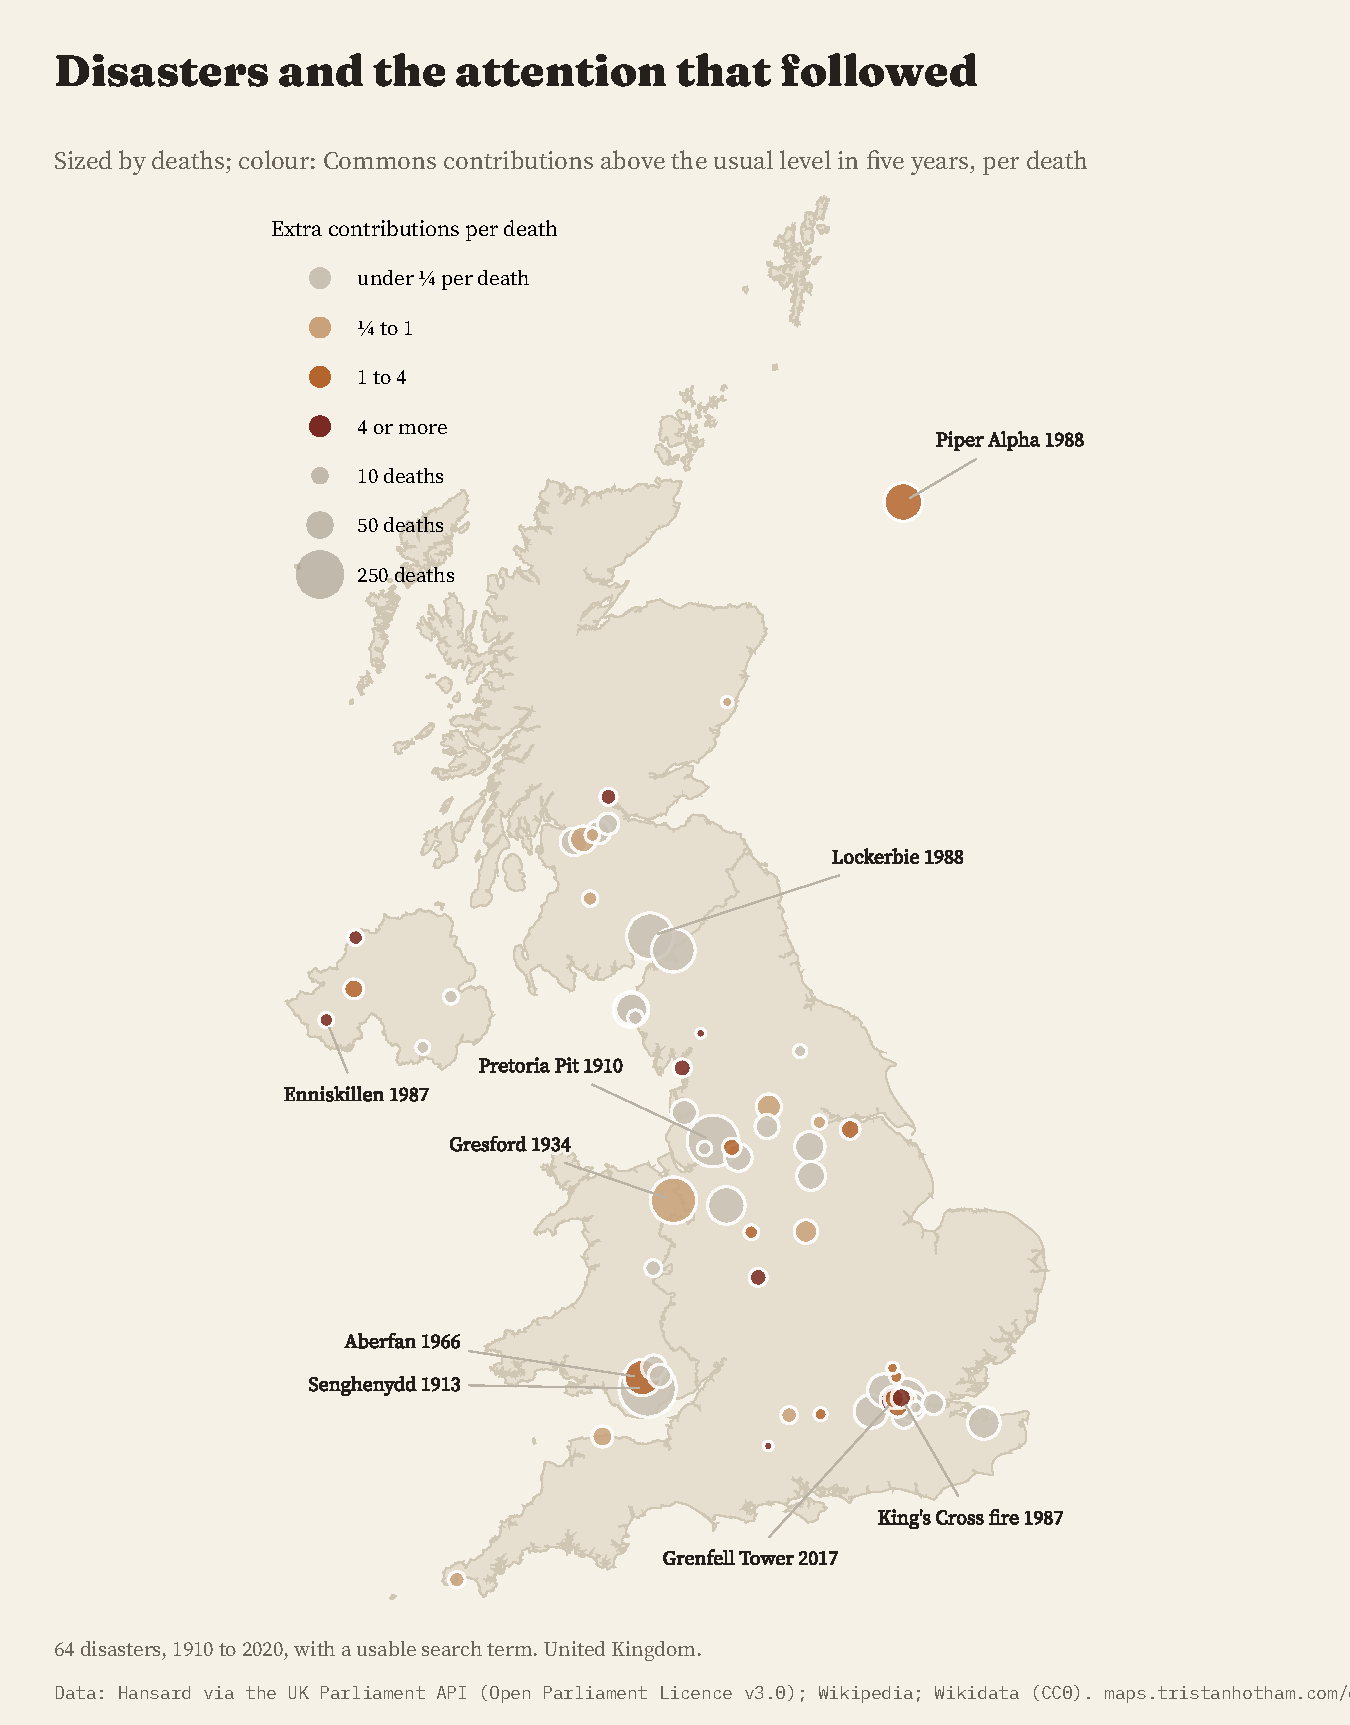
\includegraphics[width=0.78\textwidth]{f_map.pdf}
\caption{The 64 disasters in the main sample, sized by deaths and coloured by excess Commons contributions in the five years after, per death.}\label{fig:map}\end{figure}

\section{Research design}
\label{sec:design}
\subsection{Measures}
For event $e$ with search term series $n_{e,t}$ and event month $t_e$, let $k = t - t_e$ be event time. The baseline $b_e$ is the mean of $n_{e,t}$ over $k = -24, \dots, -1$ (at least 12 months). The expected count without the event is $E_{e,k} = b_e \, V_{t}/\bar V_{e}$, where $V_t$ is the volume series and $\bar V_e$ its mean over the baseline months; this scales the baseline for sittings and for the growth of Hansard. The five-year count is $C_e = \sum_{k=0}^{59} n_{e,k}$, its expectation $E_e = \sum_{k=0}^{59} E_{e,k}$ and the excess $X_e = C_e - E_e$. The peak count is $P_e = \sum_{k=0}^{2} n_{e,k}$. The time to half is the first month by which the cumulative excess reaches half of $X_e$, for events with $X_e > 0$.

\subsection{Hypotheses}
The plan set out four hypotheses and what would count against them.
\begin{description}
\item[H1 (focusing event).] Attention to the place rises after a disaster. Against: the event-study ratio for months 0 to 2 has a confidence interval including one.
\item[H2 (scaling).] Attention rises with the death toll, but less than proportionally. Against: the elasticity's interval includes zero (no scaling), or the elasticity is at least one.
\item[H3 (fading).] Attention fades quickly. Against: the median time to half of the five-year excess exceeds 12 months.
\item[H4 (whose disaster).] Conditional on deaths, kind and era: (a) disasters in London and the South East receive more attention than those elsewhere in England; (b) disasters in Scotland, Wales and Northern Ireland receive less attention in Westminster than those in England; (c) mining disasters receive less attention than other kinds, consistent with deaths treated as an occupational hazard. All tested two-sided.
\end{description}
The plan also called for heterogeneity by kind and era. Whether a public inquiry followed could not be coded consistently from the sources, so it was left out.

\subsection{Models}
The main model (M1) is a Poisson pseudo-maximum-likelihood regression \citep{SantosSilvaTenreyro2006} of the five-year count:
\begin{equation}
E[C_e] = \exp\left(\beta \log D_e + \gamma \log(1 + E_e) + \delta\,\mathrm{plain}_e + \mu_{\mathrm{kind}(e)} + \tau_{\mathrm{era}(e)}\right),
\end{equation}
where $D_e$ is the death toll, $\mathrm{plain}_e$ indicates a plain-phrase term, $\mu$ are fixed effects for six kinds (mining; transport; fire or explosion; crowd crush; bombing or shooting; other) and $\tau$ for five eras (1909 to 1938, 1939 to 1945, 1946 to 1969, 1970 to 1989, 1990 to 2021). $\beta$ is the elasticity of five-year attention with respect to deaths. Standard errors are clustered by search term (two events share a term) \citep{CameronMiller2015}. The peak model replaces $C_e$ and $E_e$ by $P_e$ and its expectation. For H4, M1 is extended with indicators for region groups (London and the South East, Scotland, Wales and Northern Ireland, against the rest of England), for nations (against England), or with a mining indicator in place of the kind effects.

The event-study model (M2) is a stacked Poisson regression of the monthly counts for $k = -24, \dots, 59$:
\begin{equation}
E[n_{e,k}] = \exp\left(\alpha_e + \textstyle\sum_{j} \theta_j \mathbf{1}[k \in B_j] + \log V_{t_e + k}\right),
\end{equation}
with event fixed effects $\alpha_e$, the log volume as an offset, and bins $B_j$: three pre-event bins ($-12$ to $-7$, $-6$ to $-4$, $-3$ to $-1$), each month from 0 to 12, and the yearly bins 13 to 24, 25 to 36, 37 to 48 and 49 to 59, with months $-24$ to $-13$ as the reference. $\exp(\theta_j)$ is the ratio of attention to its pre-event level. Events with no matching contribution in the whole window drop out. Standard errors are clustered by event; a joint Wald test of the three pre-event bins checks for pre-trends. The half-life is estimated by fitting an exponential decay to the excess ratios ($\exp\theta_j - 1$) for $k \geq 1$, with a cluster bootstrap over events (500 draws) for its interval.

\subsection{Robustness and falsification}
The plan listed the following checks. Alternative specifications: OLS of $\log(1 + \max(X_e, 0))$; PPML without kind and era effects; a negative binomial model. Sample: dropping seat-name terms; adding the ambiguous terms; dropping events whose death tolls were hand-coded; dropping wartime events; dropping bombings and shootings in Northern Ireland. Influence: leaving out each region group and each kind in turn; dropping the three largest tolls; dropping the event with the most attention. Measurement: a 36-month window; a 12-month baseline; no volume adjustment; plain-phrase terms only and ``in'' terms only; the other available term for each event; Wikidata death tolls where both sources give one. Falsification: a placebo that moves each event 36 months earlier and measures the 24 months after the false date, which end 13 months before the real event; a permutation test that shuffles death tolls across events 2,000 times; and the pre-event bins of M2.

\section{Results}
\label{sec:results}
\subsection{Descriptive patterns}
Over the five years after the 64 disasters, 6,500 Commons contributions contained the events' search terms; 60 of the events had at least one and 4 had none. The distribution is highly skewed: three events (Grenfell Tower, the Lewisham rail crash and the King's Cross fire) account for 59\% of the total, and the Lewisham count is mostly the seat-name level that the baseline removes. The raw rank correlation between deaths and five-year attention is -0.06. Figure~\ref{fig:scatter} shows why: the earliest disasters, including Senghenydd (439 deaths, 1913) and the Pretoria Pit (344 deaths, 1910), produce almost no matching contributions, as do several wartime events, while some recent disasters with few deaths were discussed at length.

\begin{figure}[tbp]\centering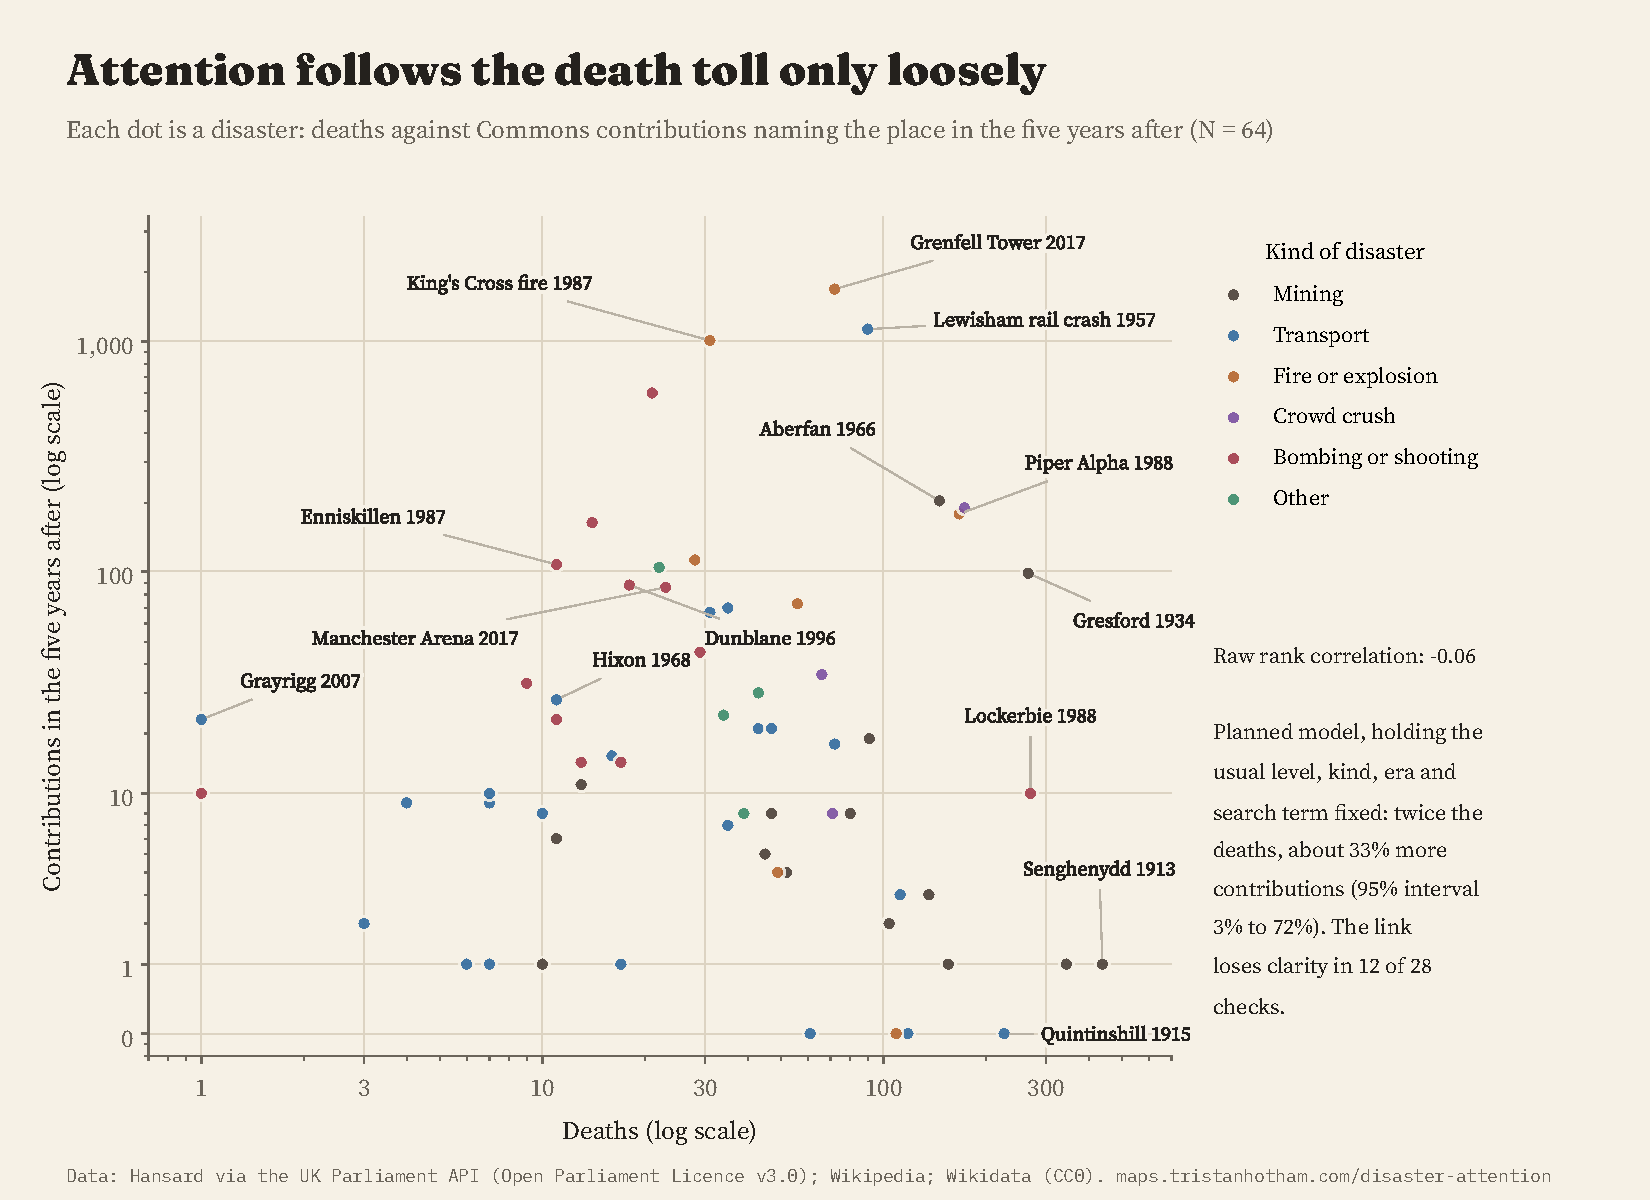
\includegraphics[width=\textwidth]{f_scatter.pdf}
\caption{Deaths against Commons contributions naming the place in the five years after, log scales, by kind of disaster ($N$ = 64).}\label{fig:scatter}\end{figure}

\subsection{H1: the rise in attention}
Figure~\ref{fig:event} and Table~\ref{tab:es} report the event study (60 events with at least one matching contribution in the window, 5,031 event-months). Before the disaster, attention is flat: the pre-event ratios lie between 0.72 and 1.03 and a joint test does not reject equality with the reference period ($\chi^2_3$ = 2.50, $p$ = 0.47). In the month of the disaster attention rises to 10.4 times the reference level (95\% CI 2.4 to 44.9), in the next month to 8.3, and in the month after that to 4.7. H1 is supported.

\begin{figure}[tbp]\centering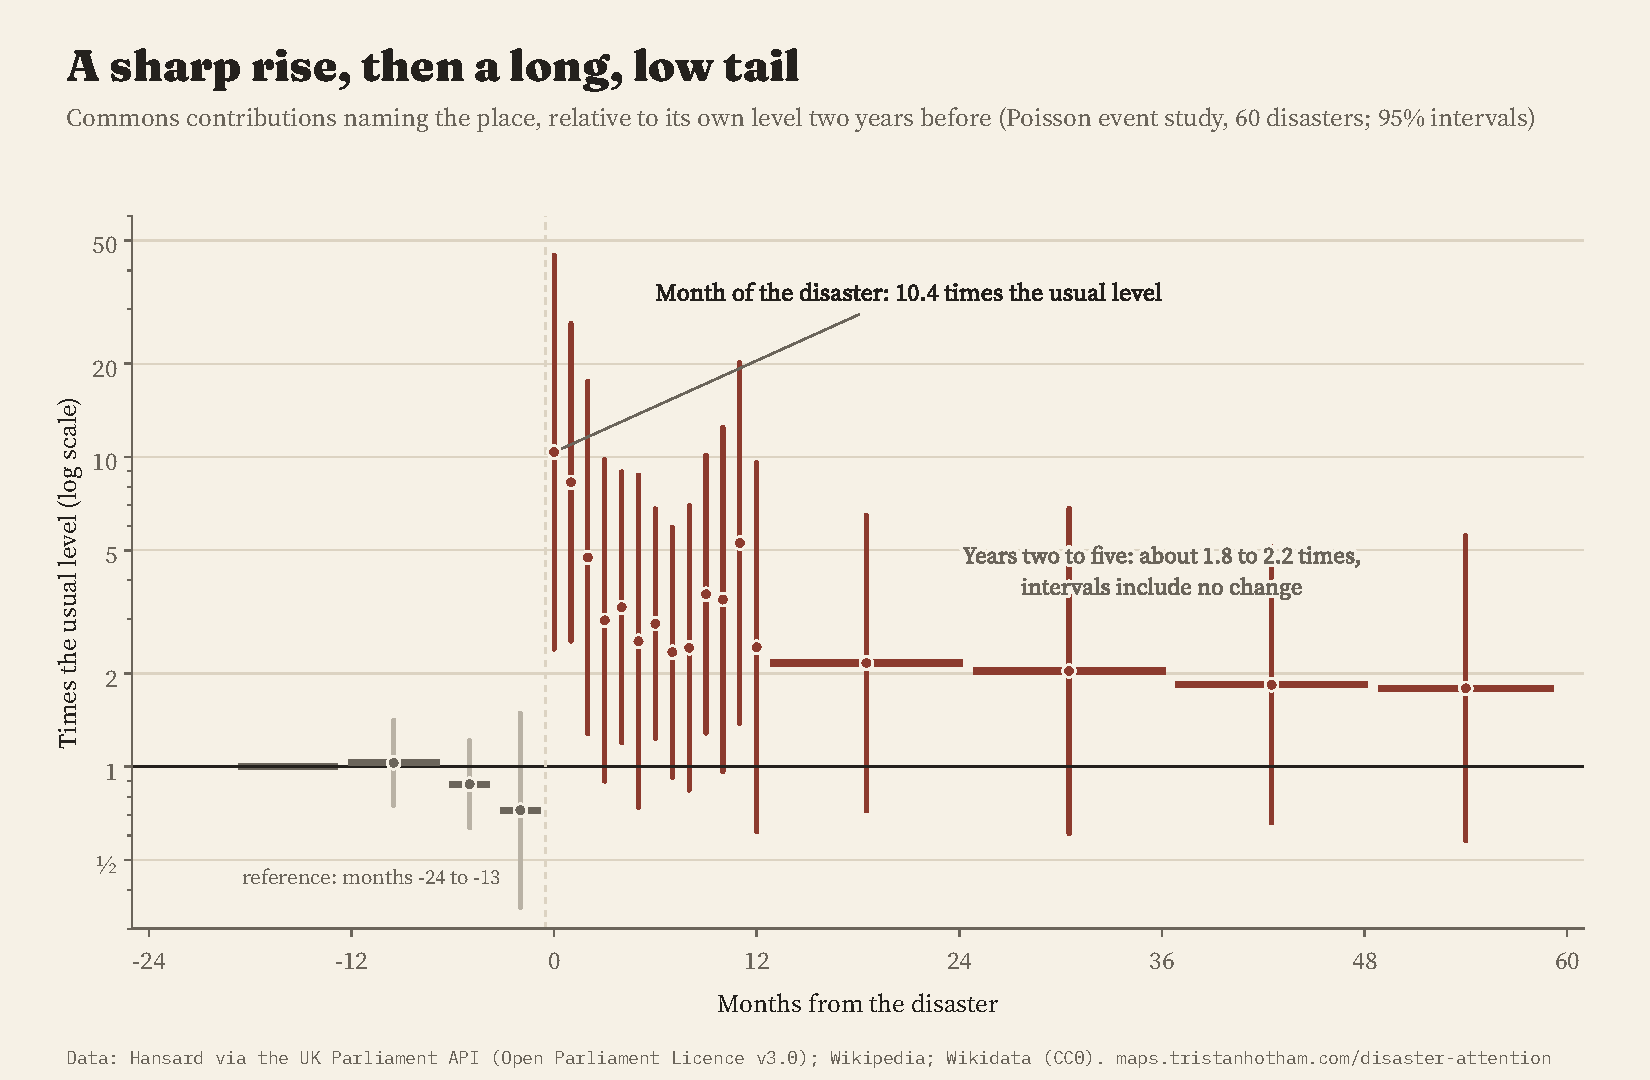
\includegraphics[width=\textwidth]{f_event.pdf}
\caption{Stacked Poisson event study (M2): Commons contributions naming the place relative to months $-24$ to $-13$, with 95\% intervals clustered by event.}\label{fig:event}\end{figure}

\subsection{H3: how fast attention fades}
The ratio falls quickly after the first months: from month 3 to month 12 it lies between 2.3 and 5.3, and from the second to the fifth year it is between 1.8 and 2.2, with intervals that all include one. The exponential fit gives a half-life of the excess ratio of 25 months, but the bootstrap interval (5 to 60 months) is too wide to be informative: the decay is fast at first and then slow, which a single exponential does not describe well, much as \citet{Candia2019} found for collective attention to cultural products.

The event-level measure is more informative (Figure~\ref{fig:half}). Among the 54 events with positive excess, the median time to half of the five-year excess is 8.5 months (interquartile range 1.2 to 22.8); 31 reached half within the first year. Under the planned criterion, H3 is supported. But the excess is not evenly spread across events: pooled across events, only 39\% of the total five-year excess came in the first year, because the events with the most attention also had the longest tails. Grenfell Tower reached half of its excess only after 23 months, Piper Alpha after 28 and Gresford after 29; each was followed by a public inquiry.

\begin{figure}[tbp]\centering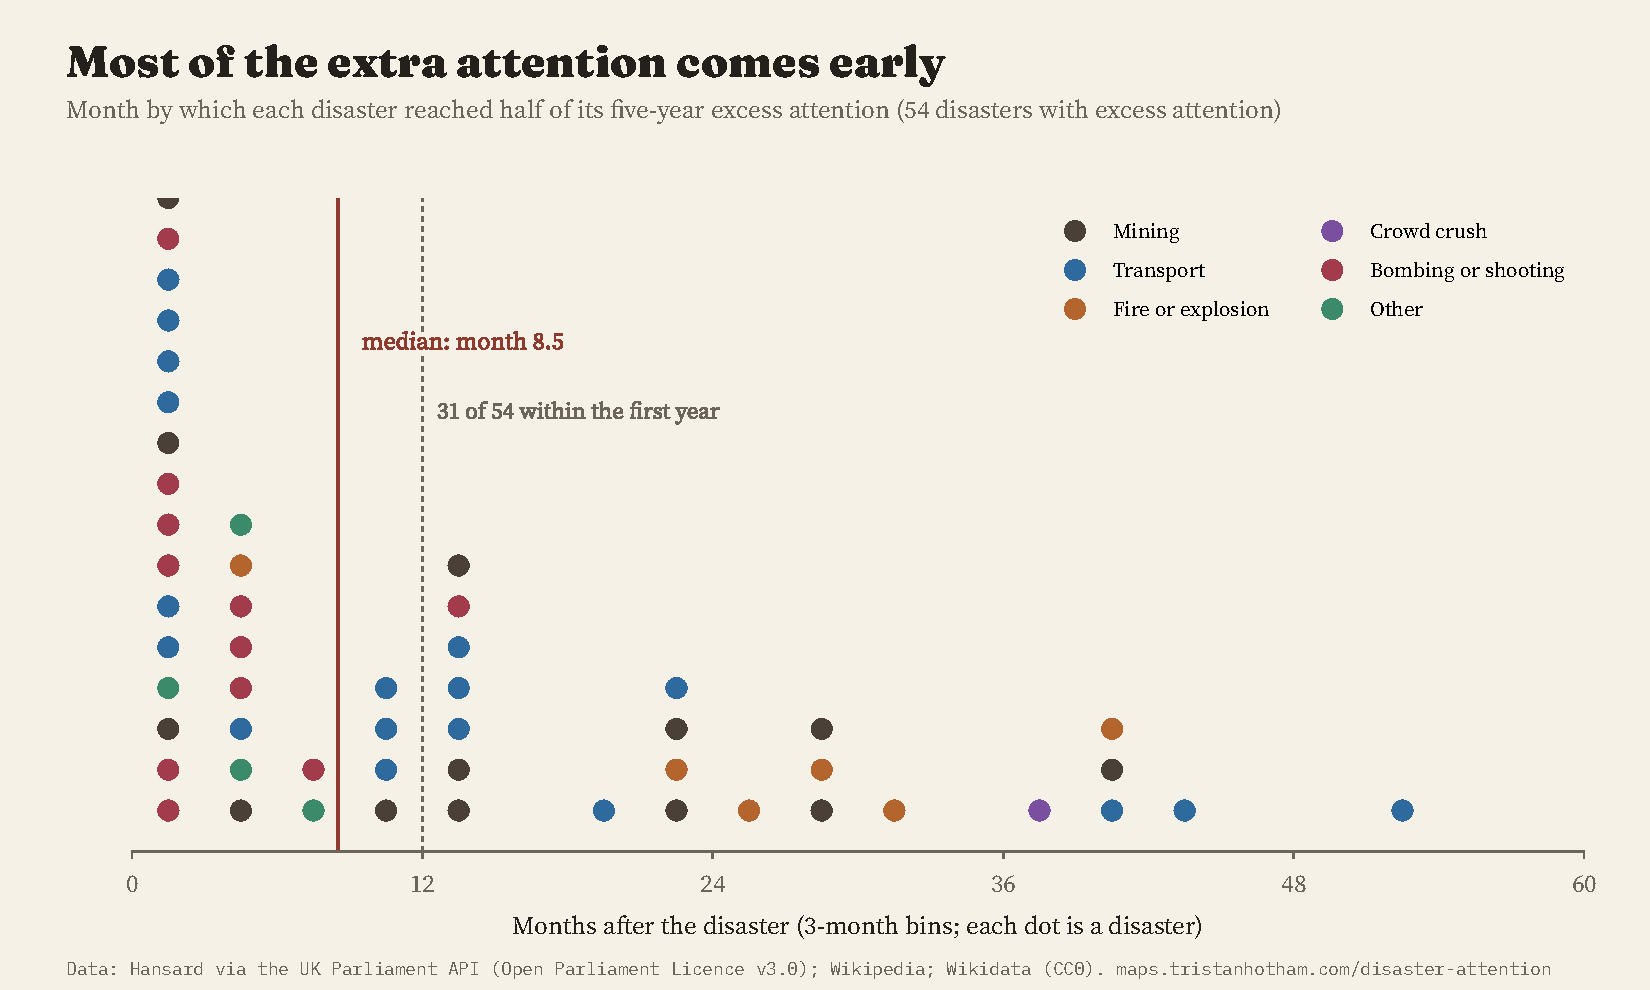
\includegraphics[width=\textwidth]{f_half.pdf}
\caption{Month by which each disaster reached half of its five-year excess attention (54 disasters with positive excess).}\label{fig:half}\end{figure}

\begin{table}[tbp]\centering\small\begin{threeparttable}\caption{Stacked Poisson event study (M2): ratio of attention to months $-24$ to $-13$.}\label{tab:es}\begin{tabular}{lrcr}\toprule Months from the disaster & Ratio & 95\% CI & $p$\\\midrule
-12 to -7 & 1.03 & [0.75, 1.41] & 0.853\\
-6 to -4 & 0.88 & [0.64, 1.22] & 0.435\\
-3 to -1 & 0.72 & [0.35, 1.49] & 0.381\\
0 & 10.37 & [2.40, 44.85] & 0.002\\
1 & 8.29 & [2.55, 26.96] & $<$0.001\\
2 & 4.74 & [1.28, 17.57] & 0.020\\
3 & 2.97 & [0.90, 9.81] & 0.074\\
4 & 3.27 & [1.20, 8.95] & 0.021\\
5 & 2.54 & [0.74, 8.73] & 0.138\\
6 & 2.90 & [1.24, 6.79] & 0.014\\
7 & 2.34 & [0.93, 5.94] & 0.072\\
8 & 2.42 & [0.84, 6.97] & 0.101\\
9 & 3.61 & [1.28, 10.14] & 0.015\\
10 & 3.47 & [0.97, 12.46] & 0.057\\
11 & 5.28 & [1.38, 20.16] & 0.015\\
12 & 2.43 & [0.62, 9.58] & 0.204\\
13 to 24 & 2.16 & [0.72, 6.48] & 0.168\\
25 to 36 & 2.04 & [0.61, 6.82] & 0.248\\
37 to 48 & 1.84 & [0.66, 5.14] & 0.244\\
49 to 59 & 1.79 & [0.58, 5.58] & 0.313\\
\bottomrule\end{tabular}\begin{tablenotes}\footnotesize\item 60 events, 5,031 event-months; event fixed effects; offset log Commons volume; standard errors clustered by event. Pre-trend test $\chi^2_3$ = 2.50, $p$ = 0.47.\end{tablenotes}\end{threeparttable}\end{table}

\subsection{H2: does attention scale with deaths?}
Table~\ref{tab:main} reports the planned model. The elasticity of five-year attention with respect to deaths is 0.42 (95\% CI 0.05 to 0.78, $p$ = 0.027, $N$ = 64): twice the deaths go with about 33\% more contributions (CI 3\% to 72\%), and ten times the deaths with about 161\% more. The expected count from the baseline is a strong predictor (elasticity 0.60), as it should be. The peak model gives a smaller elasticity of 0.24 (CI -0.07 to 0.56): the immediate response hardly varies with the toll. By the planned criterion, H2's prediction of positive but less than proportional scaling is met in the main model. As Section~\ref{sec:robust} shows, however, the positive association is fragile.

\begin{table}[tbp]\centering\small\begin{threeparttable}\caption{Planned models: Poisson (PPML) regressions of Commons contributions naming the place on log deaths.}\label{tab:main}\begin{tabular}{lrrrrrr}\toprule & \multicolumn{3}{c}{M1: five years (months 0 to 59)} & \multicolumn{3}{c}{Peak: months 0 to 2}\\\cmidrule(lr){2-4}\cmidrule(lr){5-7} Term & $b$ & (SE) & $p$ & $b$ & (SE) & $p$\\\midrule
log deaths & 0.416 & (0.188) & 0.027 & 0.243 & (0.159) & 0.126\\
log(1 + expected count) & 0.602 & (0.084) & $<$0.001 & 0.888 & (0.129) & $<$0.001\\
Plain-phrase term & 0.783 & (0.452) & 0.084 & 0.943 & (0.489) & 0.054\\
Kind: Bombing or shooting & 0.998 & (0.558) & 0.074 & 1.149 & (0.594) & 0.053\\
Kind: Crowd crush & 0.861 & (0.578) & 0.136 & 0.382 & (0.796) & 0.631\\
Kind: Fire or explosion & 2.363 & (0.472) & $<$0.001 & 2.337 & (0.472) & $<$0.001\\
Kind: Mining & 0.900 & (0.773) & 0.244 & 1.471 & (0.828) & 0.075\\
Kind: Other & -0.080 & (0.456) & 0.861 & 0.685 & (0.361) & 0.058\\
Era: 1909 to 1938 & -0.942 & (0.867) & 0.277 & -1.982 & (0.987) & 0.045\\
Era: 1939 to 1945 & -1.850 & (0.596) & 0.002 & -2.202 & (0.662) & $<$0.001\\
Era: 1946 to 1969 & 0.082 & (0.714) & 0.908 & -0.584 & (0.531) & 0.272\\
Era: 1990 to 2021 & 1.430 & (0.388) & $<$0.001 & 1.552 & (0.412) & $<$0.001\\
Constant & -0.167 & (0.775) & 0.829 & -0.699 & (0.673) & 0.299\\
\midrule $N$ & 64 & & & 64 & & \\
\bottomrule\end{tabular}\begin{tablenotes}\footnotesize\item Standard errors clustered by search term. Reference kind: transport; reference era: 1970 to 1989. The expected count is the event's own pre-event baseline scaled by Commons volume over the same months (for the peak model, months 0 to 2).\end{tablenotes}\end{threeparttable}\end{table}

The kind and era effects in Table~\ref{tab:main} are large but imprecise. Fires and explosions received about 962\% more attention than transport disasters with the same toll (CI 321 to 2580), a contrast driven by Grenfell Tower, the King's Cross fire and Flixborough. Disasters in 1990 to 2021 received 318\% more than those of 1970 to 1989 (CI 96 to 794), and wartime disasters -84\% (CI -95 to -49), consistent with reporting restrictions. Allowing the elasticity to differ before and after 1946 gives 0.37 before and 0.42 after, with no clear difference (difference 0.06, CI -1.06 to 1.17).

\subsection{H4: whose disasters?}
Table~\ref{tab:groups} and Figure~\ref{fig:groups} report the group contrasts. Conditional on deaths, kind, era and term type, disasters in London and the South East received 255\% more attention than those in the rest of England (CI 20 to 947, $p$ = 0.022), in line with H4(a). The contrasts for Scotland (12\%, CI -62 to 230), Wales (400\%, CI -7 to 2580) and Northern Ireland (-41\%, CI -80 to 80) are imprecise and include zero, as do the contrasts against all of England. H4(b) is not supported. Mining disasters did not receive clearly less attention than other kinds (250\%, CI -56 to 2675), so H4(c) is not supported either.

\begin{figure}[tbp]\centering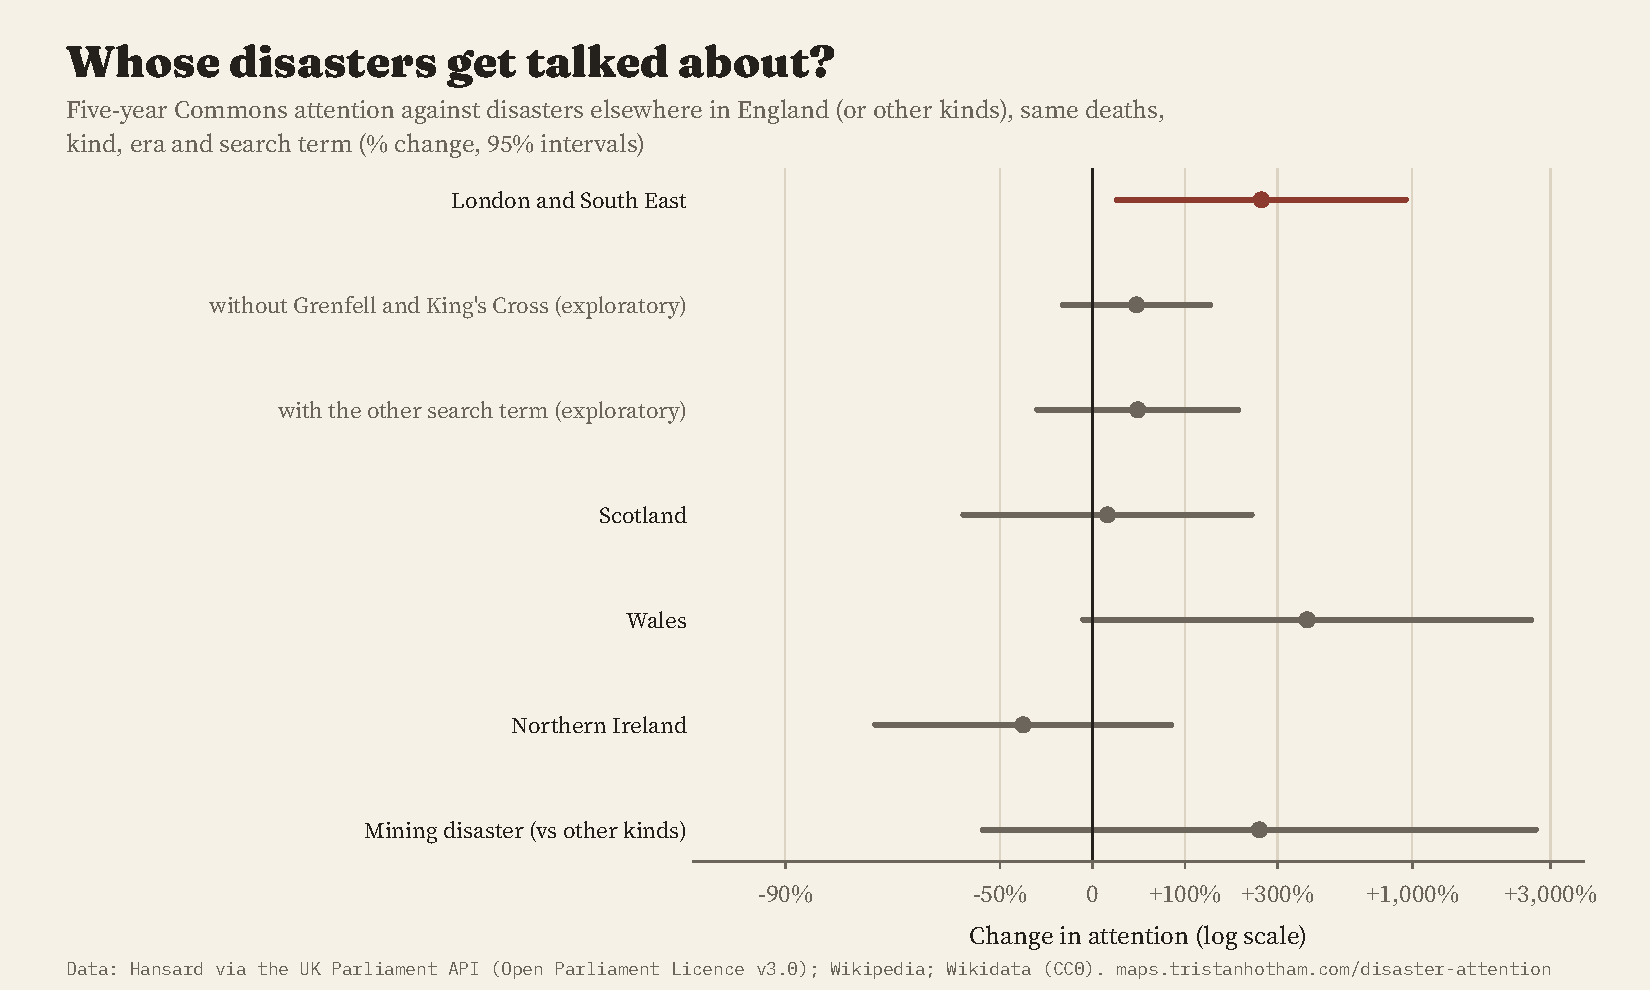
\includegraphics[width=\textwidth]{f_groups.pdf}
\caption{Group contrasts in five-year attention from M1 extended with region groups or a mining indicator (\% change, 95\% intervals). The two indented rows are exploratory.}\label{fig:groups}\end{figure}

\begin{table}[tbp]\centering\small\begin{threeparttable}\caption{H4: differences in five-year attention by region, nation and kind (\% change).}\label{tab:groups}\begin{tabular}{lrcr}\toprule & \% & 95\% CI & $p$\\\midrule
\multicolumn{4}{l}{\textit{M1 with region groups (reference: rest of England)}}\\
London and South East & 255 & [20, 947] & 0.022\\
Scotland & 12 & [-62, 230] & 0.837\\
Wales & 400 & [-7, 2580] & 0.060\\
Northern Ireland & -41 & [-80, 80] & 0.358\\
\quad elasticity in this model & 0.42 & [0.03, 0.81] & 0.033\\
\multicolumn{4}{l}{\textit{M1 with nations (reference: England)}}\\
Scotland & -17 & [-67, 107] & 0.690\\
Wales & 293 & [-21, 1866] & 0.096\\
Northern Ireland & -41 & [-81, 80] & 0.354\\
\multicolumn{4}{l}{\textit{M1 with a mining indicator in place of the kind effects}}\\
Mining & 250 & [-56, 2675] & 0.236\\
\multicolumn{4}{l}{\textit{Exploratory: the London and South East contrast}}\\
without Grenfell Tower & 184 & [11, 627] & 0.029\\
without King's Cross & 298 & [39, 1037] & 0.010\\
without both & 39 & [-20, 142] & 0.241\\
with the other search term & 40 & [-34, 198] & 0.377\\
\bottomrule\end{tabular}\begin{tablenotes}\footnotesize\item PPML with log deaths, log(1 + expected count), term type, kind and era effects as in M1; $N$ = 64; standard errors clustered by term. \% change = 100(exp($b$) $-$ 1).\end{tablenotes}\end{threeparttable}\end{table}

The London premium is not robust. In an exploratory analysis added after the planned results were seen, dropping Grenfell Tower and the King's Cross fire together reduces it to 39\% (CI -20 to 142), and using the other available search term for each event reduces it to 40\% (CI -34 to 198). Dropping any one London or South East event alone leaves it positive (15 of 15 jackknife estimates exclude zero), so the premium rests on the two together.

\section{Robustness}
\label{sec:robust}
Table~\ref{tab:robust} and Figure~\ref{fig:robust} report every planned check on the elasticity. The point estimates range from 0.10 to 0.91, all positive and all below one, but the 95\% interval includes zero in 12 of the 28 checks. The association weakens without the kind and era effects (0.10), in the OLS specification of the excess (0.13) and in the negative binomial model (0.29). It loses precision when London and the South East, Scotland, Wales, mining or transport disasters are left out, when the event with the most attention (Grenfell Tower) is dropped, and in the plain-phrase and ``in''-phrase subsamples separately. It is stronger when the three largest tolls are dropped (0.56), with a 12-month baseline (0.53), and when the hand-coded events are dropped (0.91, CI 0.10 to 1.73). Using the other available search term for each event, which moves the five-year count of the 30 swapped events from 881 to 9,433 contributions, gives 0.35 (CI 0.14 to 0.56).

The falsification tests behave as expected. The placebo, which measures attention after a false date three years before each disaster, gives an elasticity of 0.01 (CI -0.31 to 0.34, $N$ = 61). The permutation test, however, does not reject the null of no association at the 5\% level: shuffling death tolls across events gives an elasticity at least as large in absolute value in 6.9\% of 2,000 draws. Taken together, the evidence that attention scales with the death toll is weak. The robust conclusion is that the relationship, if positive, is far less than proportional.

\begin{longtable}{p{8.6cm}rcrr}\caption{Robustness: the elasticity of five-year attention with respect to deaths.}\label{tab:robust}\\\toprule Specification & $b$ & 95\% CI & $p$ & $N$\\\midrule\endfirsthead\toprule Specification & $b$ & 95\% CI & $p$ & $N$\\\midrule\endhead\bottomrule\endfoot
\multicolumn{5}{l}{\textit{Planned models}}\\
\quad Main model (M1) & 0.42 & [0.05, 0.78] & 0.027 & 64\\
\quad Peak: first three months & 0.24 & [-0.07, 0.56] & 0.126 & 64\\
\multicolumn{5}{l}{\textit{R1 Alternative specifications}}\\
\quad OLS of log(1 + excess) & 0.13 & [-0.20, 0.46] & 0.445 & 64\\
\quad PPML without type and era & 0.10 & [-0.25, 0.45] & 0.575 & 64\\
\quad Negative binomial & 0.29 & [-0.02, 0.60] & 0.068 & 64\\
\multicolumn{5}{l}{\textit{R2 Sample}}\\
\quad Drop seat-name terms & 0.41 & [0.01, 0.81] & 0.045 & 62\\
\quad Add ambiguous terms & 0.40 & [0.04, 0.76] & 0.029 & 66\\
\quad Wikipedia list and Wikidata events only & 0.91 & [0.10, 1.73] & 0.029 & 41\\
\quad Drop wartime events & 0.39 & [0.04, 0.74] & 0.031 & 58\\
\quad Drop Northern Ireland bombings and shootings & 0.38 & [0.01, 0.75] & 0.043 & 59\\
\multicolumn{5}{l}{\textit{R3 Influence}}\\
\quad Drop the three largest death tolls & 0.56 & [0.04, 1.09] & 0.035 & 61\\
\quad Drop the event with most attention & 0.28 & [-0.15, 0.70] & 0.200 & 63\\
\multicolumn{5}{l}{\textit{R3 Leave one region group out}}\\
\quad Leave out London and South East & 0.38 & [-0.11, 0.87] & 0.125 & 49\\
\quad Leave out Northern Ireland & 0.38 & [0.01, 0.75] & 0.043 & 59\\
\quad Leave out Rest of England & 0.55 & [0.16, 0.94] & 0.006 & 36\\
\quad Leave out Scotland & 0.48 & [-0.34, 1.29] & 0.249 & 54\\
\quad Leave out Wales & 0.26 & [-0.09, 0.62] & 0.149 & 58\\
\multicolumn{5}{l}{\textit{R3 Leave one kind out}}\\
\quad Leave out bombing or shooting & 0.32 & [-0.17, 0.82] & 0.200 & 52\\
\quad Leave out crowd crush & 0.40 & [0.02, 0.77] & 0.037 & 61\\
\quad Leave out fire or explosion & 0.43 & [0.01, 0.86] & 0.046 & 57\\
\quad Leave out mining & 0.27 & [-0.11, 0.64] & 0.162 & 49\\
\quad Leave out other & 0.44 & [0.06, 0.82] & 0.024 & 60\\
\quad Leave out transport & 0.46 & [-0.14, 1.06] & 0.134 & 41\\
\multicolumn{5}{l}{\textit{R4 Measurement}}\\
\quad Window 36 months & 0.44 & [0.11, 0.76] & 0.009 & 64\\
\quad Baseline 12 months & 0.53 & [0.12, 0.93] & 0.011 & 64\\
\quad No volume adjustment & 0.40 & [0.03, 0.76] & 0.032 & 64\\
\quad Plain-phrase terms only & 0.33 & [-0.22, 0.88] & 0.244 & 41\\
\quad "in" terms only & 0.14 & [-0.22, 0.49] & 0.452 & 23\\
\quad Swap to the other term where one exists & 0.35 & [0.14, 0.56] & 0.001 & 64\\
\quad Wikidata death toll where both & 0.42 & [0.05, 0.79] & 0.027 & 64\\
\multicolumn{5}{l}{\textit{R5 Falsification}}\\
\quad Placebo: fake date 36 months earlier & 0.01 & [-0.31, 0.34] & 0.932 & 61\\
\multicolumn{5}{l}{\textit{Exploratory (added after the planned results)}}\\
\quad Wikipedia list events only (40 or more deaths) & 2.02 & [0.84, 3.21] & $<$0.001 & 31\\
\quad Drop King's Cross (railway bill debates in the window) & 0.60 & [0.18, 1.01] & 0.005 & 63\\
\multicolumn{5}{l}{\textit{Search-phrase sensitivity (added in review)}}\\
\quad Disaster-specific phrase where one exists (adds Hillsborough) & 0.53 & [0.27, 0.79] & $<$0.001 & 65\\
\quad Permutation test, 2,000 shuffles of deaths & & & 0.069 & 64\\
\end{longtable}

\begin{figure}[tbp]\centering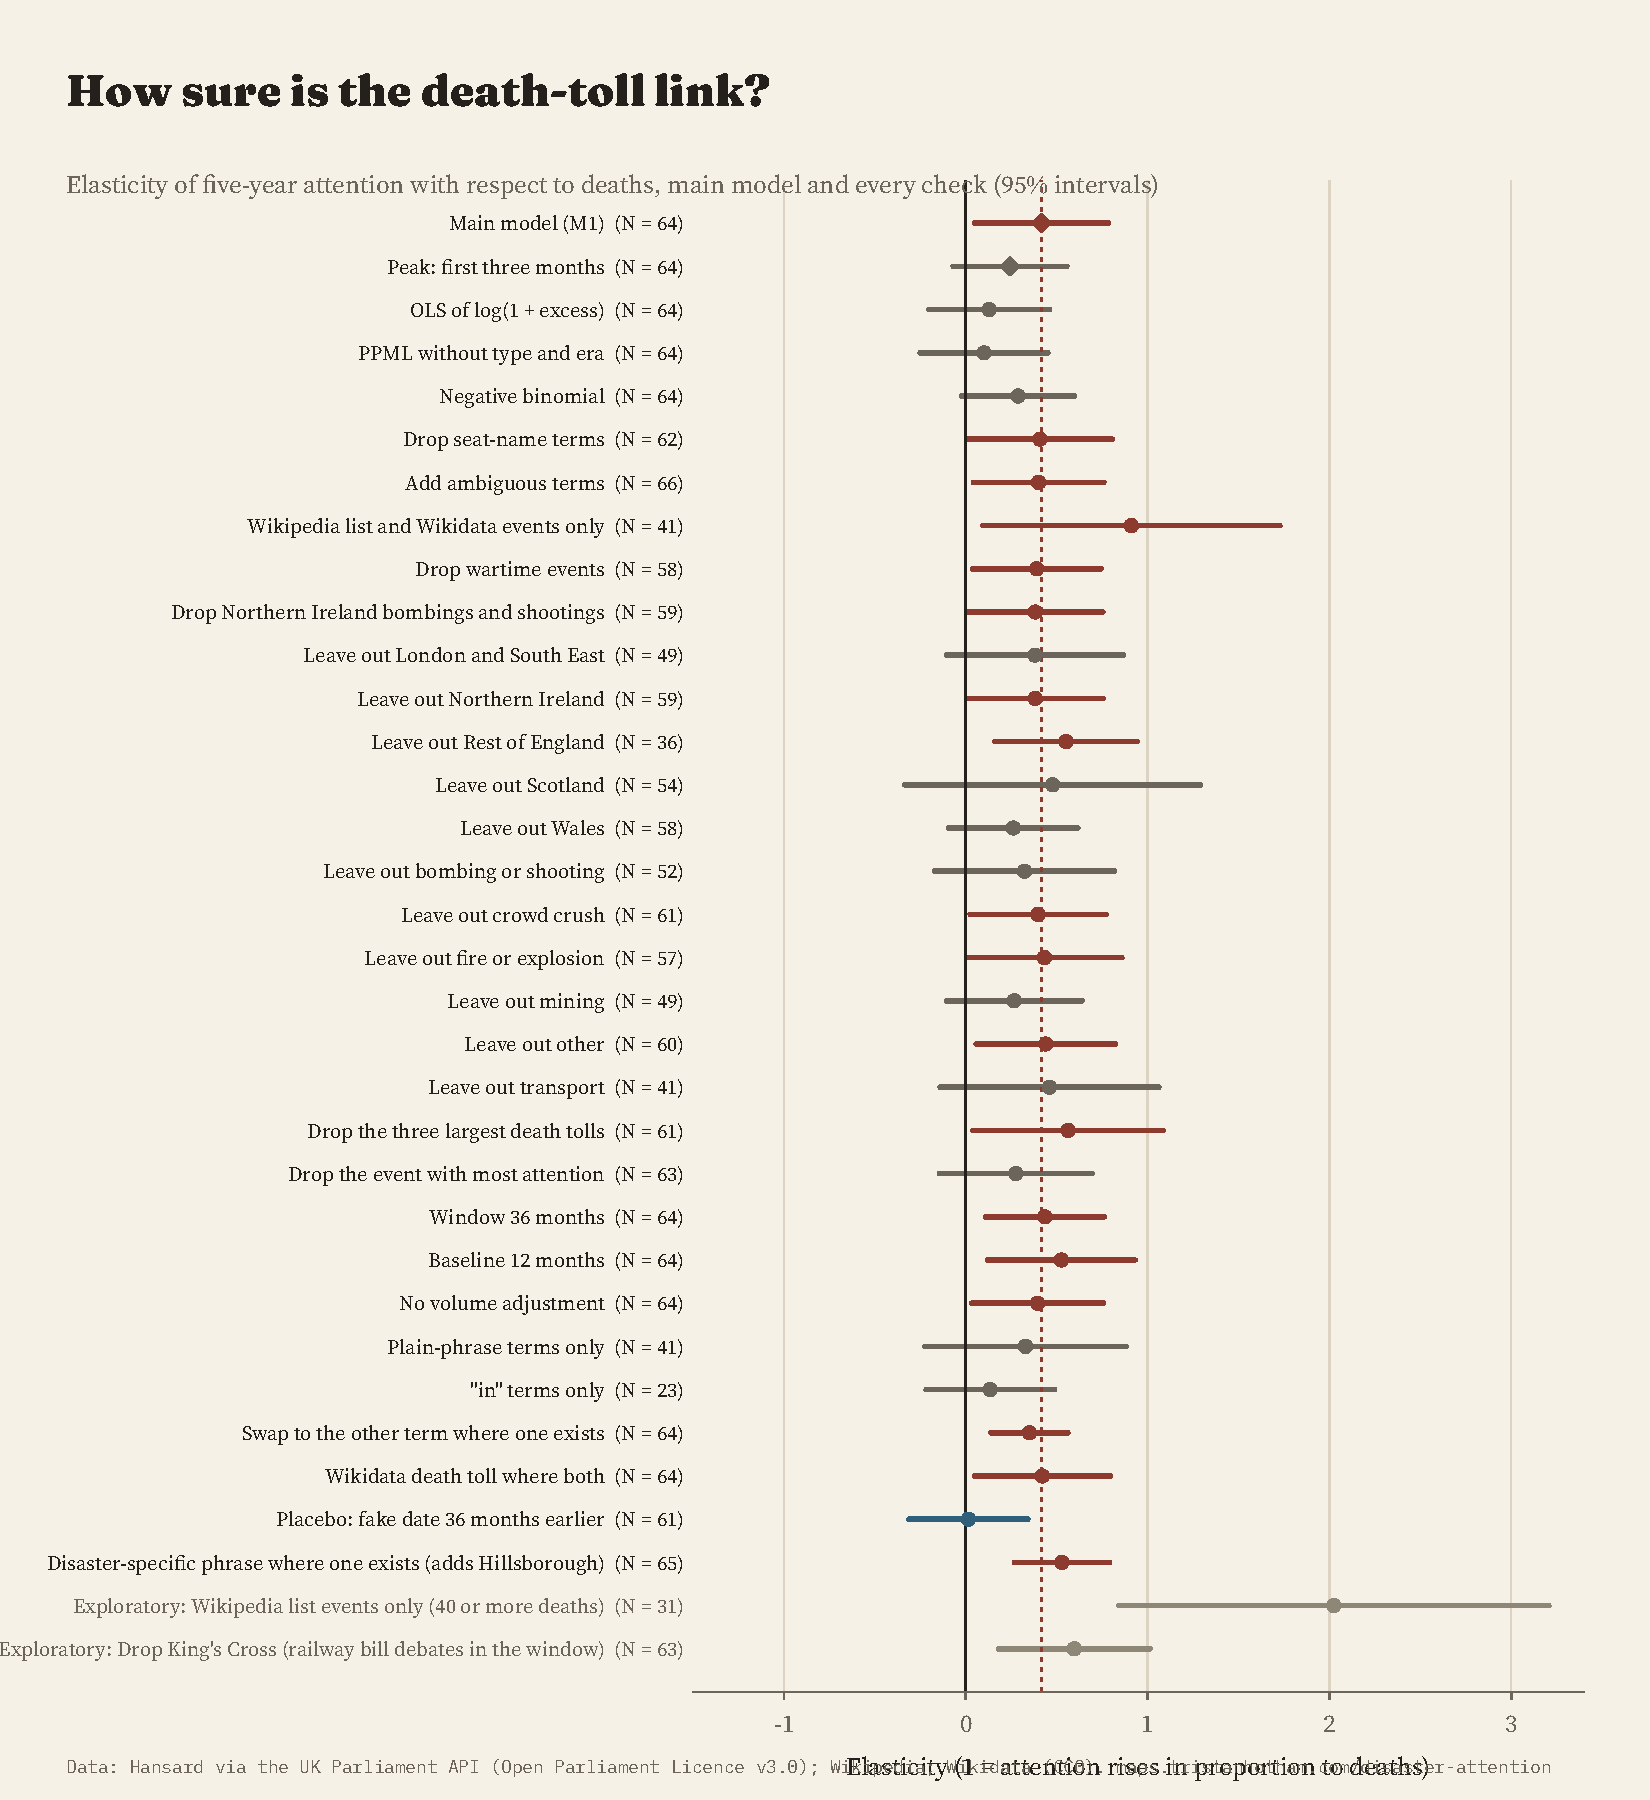
\includegraphics[width=\textwidth]{f_robust.pdf}
\caption{The elasticity of five-year attention with respect to deaths in the main model and every check (95\% intervals). Filled red: interval excludes zero.}\label{fig:robust}\end{figure}

Two exploratory checks clarify the fragility. First, ``King's Cross'' was also the subject of debates on the King's Cross Railways Bill, for the Channel Tunnel terminal, in the same years as the aftermath of the 1987 fire, a confound missed when the terms were vetted; dropping the event raises the elasticity to 0.60 (CI 0.18 to 1.01). Second, among the 31 events from the Wikipedia list alone, all with 40 or more deaths, the elasticity is 2.02 (CI 0.84 to 3.21). The events added from the harvested names, with a median of 11 deaths against 90 for the list events, were chosen because they are well known, and well-known small disasters are, almost by definition, ones that received attention. This selection flattens the estimated slope.

\begin{figure}[tbp]\centering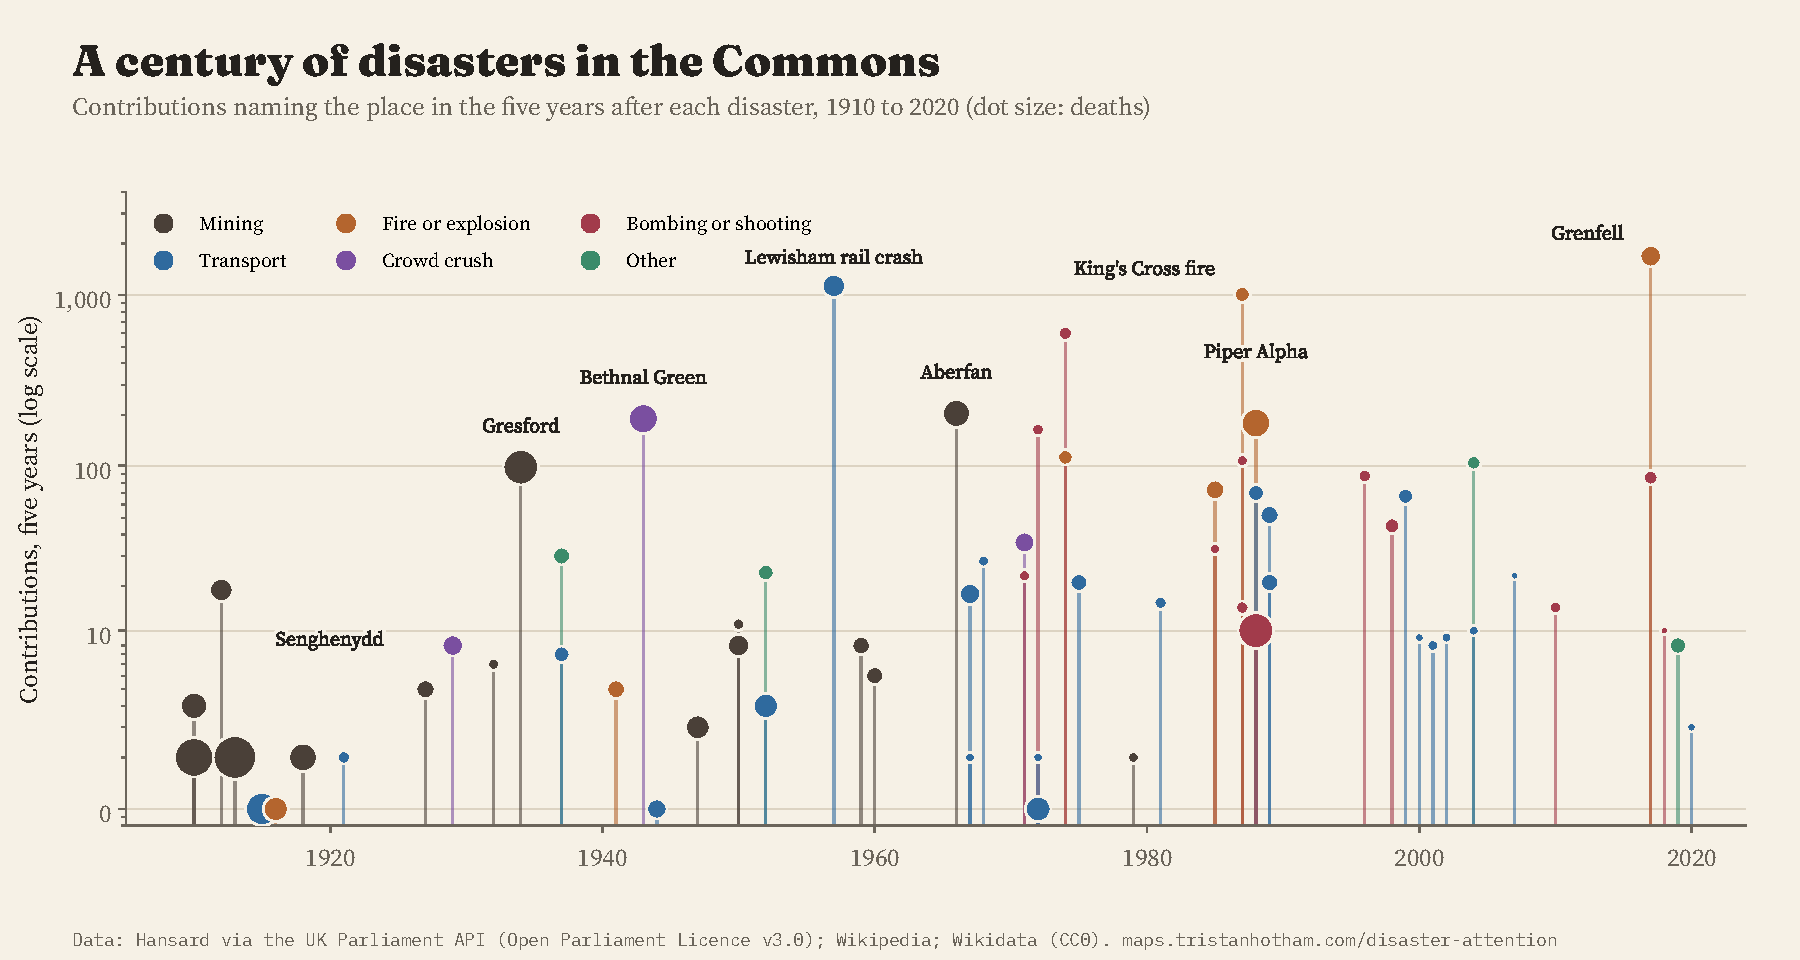
\includegraphics[width=\textwidth]{f_timeline.pdf}
\caption{Commons contributions naming the place in the five years after each disaster, by year, sized by deaths and coloured by kind.}\label{fig:timeline}\end{figure}

\section{Extension: disasters added after the first results}
\label{sec:ext}
The first version left out 26 candidates for want of a search term (Table~\ref{tab:excl} lists them as they stand after the extension). After the first results had been written up, the missing phrases were harvested from the same Hansard source, in the same form, together with disaster-specific phrases for a check of how much the search phrase matters. I applied the plan's inclusion and term rules unchanged and vetted every new term as before. Because this was done with the first results in hand, the extension is reported beside the first version, not in place of it, and the planned tables above are those of the first version.

26 candidates gained a usable term and 22 entered the main sample, with 984 deaths: among them the Easington Colliery disaster of 1951 (searched as ``Easington Colliery'', which avoids the seat name), the explosions at Chilwell and Fauld, the Llandow air crash, the Hither Green rail crash, the Droppin Well bombing at Ballykelly and the Gleision Colliery accident. Four new terms were flagged as ambiguous and enter only the check that adds ambiguous terms: Bourne End (two villages), Fernhill (several places) and McGurk and Kingsmill (also surnames in debate). Six candidates stay excluded because the only phrase available is broad or contaminated: Silvertown (a seat name from 1918), the M62 coach bombing (``M62'' names the motorway), the Hyde Park and Regent's Park bombings (the place names are broad, and ``Hyde Park bomb'' and ``Regent's Park bomb'' find 0 and 1 contributions in the five years after), the Manchester air disaster (``Manchester Airport''), the 7 July 2005 bombings (``7 July'' is a date and ``7/7'' matched 342 contributions before 2005) and the London Bridge attack of 2017. 7 of the added disasters have no matching contribution in the five years after, among them the wartime explosions at Low Moor and Fauld. One death toll was added and checked online: 18 deaths in the Markham Colliery cage accident of 1973.

Table~\ref{tab:ext} sets the two versions side by side. With 86 disasters the event study is almost unchanged (month 0 ratio 11.1, CI 2.6 to 46.4; pre-trend $p$ = 0.46), and attention fades a little faster (median time to half 5.5 months). The elasticity of five-year attention rises to 0.52 (CI 0.12 to 0.92), the peak elasticity to 0.37 (CI 0.04 to 0.71), and the permutation test now rejects no association ($p$ = 0.006, against 0.069 in the first version). The evidence for a positive, far less than proportional association is therefore stronger with the fuller list. It is still not robust: the interval includes zero in 10 of the 28 planned checks, among them the model without kind and era effects (0.11), the OLS of the excess (0.27) and dropping Grenfell Tower (0.37). The London and South East premium is 248\% (CI 22 to 893) and again falls to 29\% (CI -33 to 147) without Grenfell and King's Cross. Wales now shows a difference whose interval excludes zero (295\%, CI 11 to 1308), which the first version did not; it rests on 9 Welsh disasters, the contrast of Wales with all of England includes zero (178\%, CI -20 to 866), and it appeared only after the list was extended, so I do not treat it as a finding.

\begin{table}[tbp]\centering\small\begin{threeparttable}\caption{The first version and the extension (events added after the first results): the planned estimates side by side.}\label{tab:ext}\begin{tabular}{lcc}\toprule & First version & Extension\\\midrule
Events in the main sample & 64 & 86\\
Deaths & 4,346 & 5,330\\
Contributions in months 0 to 59 & 6,500 & 6,639\\
Events with none & 4 & 11\\
\multicolumn{3}{l}{\textit{H1 and H3: event study and fading}}\\
\quad Ratio in month 0 [95\% CI] & 10.4 [2.4, 44.9] & 11.1 [2.6, 46.4]\\
\quad Pre-trend test, $p$ & 0.47 & 0.46\\
\quad Median months to half of five-year excess & 8.5 & 5.5\\
\quad Reached half within the first year & 31 of 54 & 45 of 68\\
\multicolumn{3}{l}{\textit{H2: elasticity with respect to deaths [95\% CI]}}\\
\quad M1, five years & 0.42 [0.05, 0.78] & 0.52 [0.12, 0.92]\\
\quad Peak, months 0 to 2 & 0.24 [-0.07, 0.56] & 0.37 [0.04, 0.71]\\
\quad Permutation test, $p$ & 0.069 & 0.006\\
\quad Placebo, false date & 0.01 [-0.31, 0.34] & -0.01 [-0.30, 0.27]\\
\quad Planned checks with interval including zero & 12 of 28 & 10 of 28\\
\quad Wikipedia list events only (exploratory) & 2.02 [0.84, 3.21] & 1.96 [1.15, 2.78]\\
\quad Disaster-specific phrases (added in review) & 0.53 [0.27, 0.79] & 0.60 [0.35, 0.85]\\
\multicolumn{3}{l}{\textit{H4: \% difference [95\% CI], reference rest of England}}\\
\quad London and South East & 255 [20, 947] & 248 [22, 893]\\
\quad Scotland & 12 [-62, 230] & 36 [-53, 288]\\
\quad Wales & 400 [-7, 2580] & 295 [11, 1308]\\
\quad Northern Ireland & -41 [-80, 80] & -31 [-73, 77]\\
\quad London and South East without Grenfell and King's Cross & 39 [-20, 142] & 29 [-33, 147]\\
\quad Mining against other kinds & 250 [-56, 2675] & 155 [-39, 975]\\
\bottomrule\end{tabular}\begin{tablenotes}\footnotesize\item Same plan, models and checks; the extension adds the events that gained a usable search term (Section~\ref{sec:ext}). The London and South East row without Grenfell and King's Cross is exploratory.\end{tablenotes}\end{threeparttable}\end{table}

The search phrase itself drives the counts (Table~\ref{tab:phrase}). Disaster-specific phrases find a fraction of what the place names find: ``Grenfell Tower'' 814 contributions in five years against 1,686 for ``Grenfell'', ``King's Cross fire'' 77 against 1,009 for ``King's Cross'' (inflated by the railway bill), ``Aberfan disaster'' 52 against 203; the plain ``Lockerbie'' finds 239 against 10 for ``in Lockerbie''. Using the disaster-specific phrase for these events, which also admits Hillsborough through ``Hillsborough disaster'' (70 contributions), gives an elasticity of 0.53 (CI 0.27 to 0.79) in the first version and 0.60 (CI 0.35 to 0.85) with the extension. This check was added in review, after the results were known.

\begin{table}[tbp]\centering\small\begin{threeparttable}\caption{How the search phrase drives the counts: the study's term and a disaster-specific phrase, contributions in months 0 to 59.}\label{tab:phrase}\begin{tabular}{lrrlrr}\toprule Disaster & Study term & $C$ & Disaster-specific phrase & $C$ & Months 0 to 2\\\midrule
Grenfell Tower fire & Grenfell & 1,686 & Grenfell Tower & 814 & 210\\
King's Cross fire & King's Cross & 1,009 & King's Cross fire & 77 & 11\\
Hillsborough disaster & Hillsborough & 400 & Hillsborough disaster & 70 & 28\\
Aberfan disaster & Aberfan & 203 & Aberfan disaster & 52 & 15\\
Gresford disaster & Gresford & 98 & Gresford disaster & 13 & 1\\
Clapham Junction rail crash & Clapham Junction & 69 & Clapham rail & 19 & 1\\
Moorgate tube crash & Moorgate & 20 & Moorgate disaster & 2 & 2\\
Lockerbie (Pan Am Flight 103) & in Lockerbie & 10 & Lockerbie & 239 & 68\\
\bottomrule\end{tabular}\begin{tablenotes}\footnotesize\item Same source and measure. Hillsborough is excluded from the main sample as ambiguous; ``Hillsborough disaster'' is not. Added in review, after the first results.\end{tablenotes}\end{threeparttable}\end{table}

\section{Discussion}
\label{sec:discussion}
\subsection{What the results show}
The first finding is the shape of attention. In the month of a disaster, Commons attention to the place jumps by an order of magnitude; for most events it falls back within months. This is the pattern Kingdon and Birkland describe for focusing events, and the early stages of Downs's cycle. The tail is the more interesting part. Averaged across events, attention in years two to five stays about twice its earlier level, although each yearly estimate is imprecise, and the events with most attention overall are those whose aftermath lasted longest. Grenfell Tower, Piper Alpha and Gresford all reached half of their five-year excess only after about two years. Parliament returned to them because there was something to return to: an inquiry, a prosecution, legislation or a campaign. This is consistent with accounts that see the post-crisis period as a contest over accountability \citep{Boin2009,Hood2011} and with case studies of Aberfan and Hillsborough \citep{McLeanJohnes2000,Scraton1999}. The data cannot show that the inquiry caused the attention: both may follow from the scale or the visibility of the failure.

The second finding is that the death toll explains little. The raw rank correlation is close to zero, and conditional on the usual level of mentions, kind and era the elasticity is about 0.42 in the planned model and is not robust. Two mechanisms are consistent with this. One is the psychophysical numbing documented in experiments \citep{Fetherstonhaugh1997,Slovic2007}: legislators, like others, may respond to the fact of a disaster more than to its size. The other is that the political salience of a disaster depends on what it reveals: a failure of regulation, a public body under question, a group of bereaved families organising. Several rail accidents that raised questions about safety regimes drew tens of contributions despite modest tolls: Grayrigg (1 death, 22 contributions in five years), Hixon (11 deaths, 27), Ladbroke Grove (31, 66) and Clapham Junction (35, 69). The study cannot separate these mechanisms.

The third finding concerns location. There is a London and South East premium in the planned model, but it rests on two London disasters and disappears without them or with other search terms. With so few events in each region, the data cannot rule out moderate differences in either direction, and they give no support to the view that disasters in Scotland, Wales, Northern Ireland or in mining communities were systematically ignored in the Commons. The absence of evidence here is not evidence of equal treatment: the confidence intervals are wide.

\subsection{Lists, words and the filter of memory}
The most general lesson concerns the sources. Any list of disasters is a record of what has been remembered. The Wikipedia list uses a threshold of 40 deaths; smaller disasters enter this study only through Wikidata or through a list of names that are already well known. The harvested names include the rail crashes of the privatised railway, the Morecambe Bay cockling deaths and the Dunblane and Hungerford shootings, all small by death toll and all prominent in public memory, partly because of the political response that followed. Including them flattens the relationship between deaths and attention, and excluding them steepens it sharply. This is selection on the outcome, and the paper cannot remove it with the available data; a complete register of fatal incidents would be needed.

The words used to search the record are a second filter. People in Parliament refer to ``the Lockerbie bombing'' and ``the Hillsborough disaster'' more than to events ``in Lockerbie''; the ``in'' phrase for Lockerbie finds 10 contributions in five years, the plain word 239. Some names have other meanings in debate, which this study handled by vetting, flagging and robustness checks, but at least one confound (King's Cross) was found only after the results. And the searchable record itself changes over time: few contributions from the 1910s match even the names of disasters that killed hundreds, which probably reflects the indexing of older volumes and wartime restrictions as much as the attention paid at the time. Studies that use Hansard text search over long periods, including studies of members' activity \citep{EggersSpirling2014}, should treat early counts with similar care.

\subsection{Limitations}
The design is observational. The death toll is not assigned at random, and disasters with larger tolls differ in many ways from those with smaller ones. The measure counts contributions that contain a phrase; it does not measure the content, tone or consequences of what was said, and much of the response to a disaster takes place outside the chamber, in inquiries, courts, local government and communities. The event list is incomplete and selected, as discussed above, and even after the extension 13 candidates could not be studied, 6 of them for want of a specific search term. The House of Lords, written questions and select committees are not included. The volume adjustment is approximate. Death tolls are as recorded in the sources, which sometimes include perpetrators and sometimes differ. Finally, the sample is small: with 64 events, contrasts between regions or kinds rest on a handful of cases.

\section{Conclusion}
\label{sec:conclusion}
Parliament does notice disasters. The Commons names the place far more often in the month a disaster happens, and for most disasters that attention fades within the year. Some disasters hold Parliament's attention for years, usually those that are followed by inquiries and campaigns. How many people died explains little of the variation: attention rises with the toll far less than proportionally, a little more clearly once the later-searchable disasters are added, but not robustly; and the evidence that attention depends on where the disaster happened is weak once two London disasters are set aside. The study also shows how much the answers depend on which disasters are remembered and on the words used to find them, which are themselves products of the attention being measured. A complete register of fatal disasters and searches of the full text of debates would allow these questions to be answered with more confidence.

\section*{Data availability}
Data and code: Zenodo DOI https://doi.org/10.5281/zenodo.24094466. The repository (\url{https://github.com/Tristan-Hotham/disaster-attention}) contains the curated event list with inclusion decisions and sources, the monthly event panel, the model outputs, every number reported here in a single results file, and the code that reproduces all of it from the raw Hansard counts, the Wikipedia list and Wikidata. The interactive version is at \url{https://maps.tristanhotham.com/disaster-attention/}.

\section*{AI statement}
I wrote the text, with drafting and editing assistance from Claude (Anthropic), which also helped prepare the analysis code. I reviewed and checked all text and results.

\bibliographystyle{plainnat}
\bibliography{refs}

\appendix
\section{Appendix}
\label{sec:appendix}
\subsection{Event list and exclusions}
Table~\ref{tab:events} lists every event in the main sample with its search term, baseline and counts. Table~\ref{tab:excl} lists the candidates that were excluded, with the reason and, where relevant, the search term that would be needed to include them. Deaths hand-coded from Wikipedia articles were checked online in 2026: Abermule (17), Castlecary (35), Lynmouth (34), Thirsk (7), Hixon (11), Eltham Well Hall (6), Flixborough (28), Golborne (10), Cardowan (11, 1932), Penlee (16), King's Cross (31), Enniskillen (11 on the day; a twelfth person died in 2000), Clapham Junction (35), Ladbroke Grove (31), Hatfield (4), Great Heck (10), Potters Bar (7), Morecambe Bay (at least 22), Ufton Nervet (7), Grayrigg (1), Ballymurphy (11), Amesbury (1) and Carmont (3); in the extension, Gleision (4) and the Markham Colliery cage accident of 1973 (18).

{\footnotesize\begin{longtable}{p{5.2cm}lrlrrrrr}\caption{The 86 disasters in the main sample of the extension ($^x$: added in the extension, Section~\ref{sec:ext}; the other 86 form the main sample of the first version).}\label{tab:events}\\\toprule Disaster & Month & Deaths & Search term & Base & $C$ & $E$ & $P$ & Half\\\midrule\endfirsthead\toprule Disaster & Month & Deaths & Search term & Base & $C$ & $E$ & $P$ & Half\\\midrule\endhead\bottomrule\multicolumn{9}{p{15cm}}{\footnotesize Base: mean monthly contributions in months $-24$ to $-1$. $C$: contributions in months 0 to 59; $E$: expected at the usual level; $P$: months 0 to 2; Half: month by which half the five-year excess was reached. $^h$ death toll from the event's Wikipedia article, checked by hand. $^s$ also a Commons seat name throughout the window. $^x$ added in the extension.}\\\endlastfoot
Wellington Pit disaster & 1910-05 & 136 & Wellington Pit & 0.00 & 3 & 0.0 & 3 & 1\\
Pretoria Pit disaster (Hulton Colliery) & 1910-12 & 344 & Pretoria Pit & 0.00 & 1 & 0.0 & 0 & 3\\
Cadeby Main pit disaster & 1912-07 & 91 & Cadeby & 0.00 & 18 & 0.0 & 1 & 12\\
Senghenydd colliery disaster & 1913-10 & 439 & Senghenydd & 0.00 & 1 & 0.0 & 0 & 9\\
Quintinshill rail crash & 1915-05 & 226 & Quintinshill & 0.00 & 0 & 0.0 & 0 & \\
Faversham gunpowder mill explosion & 1916-04 & 109 & in Faversham & 0.00 & 0 & 0.0 & 0 & \\
Low Moor explosion & 1916-08 & 40 & Low Moor$^x$ & 0.00 & 0 & 0.0 & 0 & \\
Minnie Pit disaster & 1918-01 & 155 & Minnie Pit & 0.00 & 1 & 0.0 & 0 & 23\\
Chilwell shell filling factory explosion & 1918-07 & 137 & Chilwell$^x$ & 0.00 & 7 & 0.0 & 1 & 11\\
Abermule train collision & 1921-01 & 17$^h$ & Abermule & 0.00 & 1 & 0.0 & 1 & 1\\
R38 airship crash (Hull) & 1921-08 & 44 & R.38$^x$ & 0.08 & 2 & 6.7 & 0 & \\
Marine Colliery disaster (Cwm) & 1927-03 & 52 & in Ebbw Vale & 0.00 & 4 & 0.0 & 0 & 12\\
Glen Cinema disaster & 1929-12 & 71 & in Paisley & 0.17 & 8 & 12.3 & 2 & \\
Bentley Colliery disaster & 1931-11 & 45 & Bentley Colliery$^x$ & 0.00 & 3 & 0.0 & 1 & 6\\
Cardowan Colliery explosion & 1932-11 & 11$^h$ & Cardowan & 0.00 & 6 & 0.0 & 3 & 0\\
Gresford disaster & 1934-09 & 266 & Gresford & 0.00 & 98 & 0.0 & 6 & 29\\
Wharncliffe Woodmoor colliery disaster & 1936-08 & 58 & Wharncliffe Woodmoor$^x$ & 0.00 & 6 & 0.0 & 0 & 11\\
Croydon typhoid outbreak & 1937-10 & 43 & in Croydon & 0.38 & 29 & 18.6 & 6 & 5\\
Castlecary rail disaster & 1937-12 & 35$^h$ & Castlecary & 0.00 & 7 & 0.0 & 2 & 3\\
Markham Colliery disaster & 1938-05 & 79 & Markham Colliery$^x$ & 0.08 & 7 & 3.2 & 5 & 0\\
Valleyfield mining disaster & 1939-10 & 35 & Valleyfield$^x$ & 0.00 & 5 & 0.0 & 1 & 10\\
Booth's clothing factory fire & 1941-10 & 49 & in Huddersfield & 0.00 & 4 & 0.0 & 0 & 30\\
Sneyd Colliery disaster & 1942-01 & 57 & Sneyd$^x$ & 0.00 & 6 & 0.0 & 5 & 1\\
Bethnal Green tube station crush & 1943-03 & 173 & Bethnal Green$^s$ & 3.54 & 189 & 306.7 & 10 & \\
Freckleton air disaster & 1944-08 & 61 & in Freckleton & 0.00 & 0 & 0.0 & 0 & \\
RAF Fauld explosion & 1944-11 & 70 & Fauld$^x$ & 0.00 & 0 & 0.0 & 0 & \\
Burngrange mining disaster & 1947-01 & 15 & Burngrange$^x$ & 0.00 & 0 & 0.0 & 0 & \\
William Pit disaster & 1947-08 & 104 & in Whitehaven & 0.04 & 2 & 3.4 & 2 & \\
Llandow air disaster & 1950-03 & 80 & Llandow$^x$ & 0.00 & 5 & 0.0 & 2 & 3\\
Knockshinnoch disaster & 1950-09 & 13 & Knockshinnoch & 0.00 & 11 & 0.0 & 2 & 40\\
Creswell Colliery disaster & 1950-09 & 80 & Creswell & 0.00 & 8 & 0.0 & 0 & 22\\
Easington Colliery disaster & 1951-05 & 81 & Easington Colliery$^x$ & 0.00 & 3 & 0.0 & 2 & 0\\
Lynmouth flood & 1952-08 & 34$^h$ & Lynmouth & 0.00 & 23 & 0.0 & 1 & 7\\
Harrow and Wealdstone rail crash & 1952-10 & 112 & Harrow and Wealdstone & 0.00 & 3 & 0.0 & 3 & 0\\
Aquila Airways flying boat crash (Isle of Wight) & 1957-11 & 45 & Chessell$^x$ & 0.00 & 0 & 0.0 & 0 & \\
Lewisham rail crash & 1957-12 & 90 & Lewisham$^s$ & 24.21 & 1130 & 1639.9 & 84 & \\
Auchengeich mining disaster & 1959-09 & 47 & Auchengeich & 0.00 & 8 & 0.0 & 4 & 2\\
Six Bells colliery disaster & 1960-06 & 45 & Six Bells & 0.17 & 5 & 11.1 & 2 & \\
Little Baldon air crash & 1965-07 & 41 & Little Baldon$^x$ & 0.00 & 0 & 0.0 & 0 & \\
Penmaenpool ferry disaster & 1966-07 & 15 & Penmaenpool$^x$ & 0.00 & 0 & 0.0 & 0 & \\
Aberfan disaster & 1966-10 & 146 & Aberfan & 0.00 & 203 & 0.0 & 48 & 14\\
Stockport air disaster & 1967-06 & 72 & in Stockport & 0.17 & 17 & 10.7 & 0 & 44\\
Thirsk rail crash & 1967-07 & 7$^h$ & in Thirsk & 0.00 & 1 & 0.0 & 0 & 51\\
Hither Green rail crash & 1967-11 & 49 & Hither Green$^x$ & 0.08 & 25 & 5.8 & 7 & 4\\
Hixon rail crash & 1968-01 & 11$^h$ & Hixon & 0.00 & 27 & 0.0 & 6 & 10\\
Ibrox disaster & 1971-01 & 66 & Ibrox & 0.00 & 35 & 0.0 & 2 & 36\\
Ballymurphy killings & 1971-08 & 11$^h$ & Ballymurphy & 0.75 & 22 & 56.7 & 0 & \\
Bloody Sunday (Derry) & 1972-01 & 14 & in Londonderry & 1.38 & 163 & 99.6 & 26 & 4\\
Eltham Well Hall rail crash & 1972-06 & 6$^h$ & Eltham Well Hall & 0.00 & 1 & 0.0 & 1 & 0\\
Staines air disaster (BEA Flight 548) & 1972-06 & 118 & in Staines & 0.00 & 0 & 0.0 & 0 & \\
Claudy bombing & 1972-07 & 9 & Claudy$^x$ & 0.00 & 6 & 0.0 & 4 & 0\\
Markham Colliery cage accident & 1973-07 & 18$^h$ & Markham Colliery$^x$ & 0.00 & 5 & 0.0 & 0 & 6\\
Flixborough disaster & 1974-06 & 28$^h$ & Flixborough & 0.00 & 112 & 0.0 & 54 & 5\\
Birmingham pub bombings & 1974-11 & 21 & in Birmingham & 7.71 & 597 & 492.2 & 84 & 1\\
Moorgate tube crash & 1975-02 & 43 & Moorgate & 0.08 & 20 & 5.5 & 8 & 2\\
Golborne Colliery explosion & 1979-03 & 10$^h$ & in Golborne & 0.00 & 1 & 0.0 & 0 & 27\\
Denmark Place fire & 1980-08 & 37 & Denmark Place$^x$ & 0.00 & 0 & 0.0 & 0 & \\
Penlee lifeboat disaster & 1981-12 & 16$^h$ & Penlee & 0.00 & 15 & 0.0 & 3 & 12\\
Droppin Well bombing (Ballykelly) & 1982-12 & 17 & Ballykelly$^x$ & 0.04 & 35 & 2.7 & 20 & 0\\
Newry mortar attack & 1985-02 & 9 & in Newry & 0.46 & 32 & 30.8 & 4 & 1\\
Bradford City stadium fire & 1985-05 & 56 & Bradford City & 0.33 & 72 & 23.0 & 14 & 41\\
Hungerford shootings & 1987-08 & 17 & in Hungerford & 0.00 & 14 & 0.0 & 5 & 4\\
Enniskillen bombing & 1987-11 & 11$^h$ & Enniskillen & 0.17 & 107 & 10.9 & 40 & 4\\
King's Cross fire & 1987-11 & 31$^h$ & King's Cross & 0.50 & 1009 & 32.7 & 106 & 24\\
Piper Alpha & 1988-07 & 167 & Piper Alpha & 0.00 & 178 & 0.0 & 14 & 28\\
Ballygawley bus bombing & 1988-08 & 8 & Ballygawley$^x$ & 0.00 & 9 & 0.0 & 0 & 5\\
Clapham Junction rail crash & 1988-12 & 35$^h$ & Clapham Junction & 0.04 & 69 & 2.3 & 19 & 12\\
Lockerbie (Pan Am Flight 103) & 1988-12 & 270 & in Lockerbie & 0.04 & 10 & 2.3 & 7 & 0\\
Kegworth air disaster & 1989-01 & 47 & Kegworth & 0.04 & 20 & 2.3 & 13 & 1\\
Marchioness disaster & 1989-08 & 51 & Marchioness & 0.00 & 51 & 0.0 & 0 & 20\\
Dunblane school shooting & 1996-03 & 18 & in Dunblane & 0.04 & 87 & 2.7 & 21 & 8\\
Omagh bombing & 1998-08 & 29 & in Omagh & 0.08 & 44 & 5.2 & 24 & 1\\
Ladbroke Grove rail crash & 1999-10 & 31$^h$ & Ladbroke Grove & 0.17 & 66 & 10.5 & 22 & 9\\
Hatfield rail crash & 2000-10 & 4$^h$ & in Hatfield & 0.00 & 9 & 0.0 & 0 & 39\\
Great Heck rail crash & 2001-02 & 10$^h$ & Great Heck & 0.00 & 8 & 0.0 & 4 & 1\\
Potters Bar rail crash & 2002-05 & 7$^h$ & in Potters Bar & 0.00 & 9 & 0.0 & 4 & 9\\
Morecambe Bay cockling disaster & 2004-02 & 22$^h$ & Morecambe Bay & 0.21 & 104 & 14.0 & 40 & 3\\
Ufton Nervet rail crash & 2004-11 & 7$^h$ & Ufton Nervet & 0.00 & 10 & 0.0 & 7 & 1\\
Grayrigg derailment & 2007-02 & 1$^h$ & Grayrigg & 0.00 & 22 & 0.0 & 7 & 23\\
Cumbria shootings & 2010-06 & 13 & in Whitehaven & 0.17 & 14 & 13.6 & 4 & 0\\
Gleision Colliery accident & 2011-09 & 4$^h$ & Gleision$^x$ & 0.00 & 15 & 0.0 & 10 & 1\\
Manchester Arena bombing & 2017-05 & 23 & Manchester Arena & 0.00 & 85 & 0.0 & 9 & 14\\
Grenfell Tower fire & 2017-06 & 72 & Grenfell & 0.08 & 1686 & 4.7 & 259 & 23\\
Amesbury Novichok poisoning & 2018-07 & 1$^h$ & in Amesbury & 0.00 & 10 & 0.0 & 7 & 2\\
Essex lorry deaths (Grays) & 2019-10 & 39 & in Grays & 0.00 & 8 & 0.0 & 5 & 0\\
Carmont derailment & 2020-08 & 3$^h$ & Carmont & 0.00 & 2 & 0.0 & 0 & 13\\
\end{longtable}}

{\footnotesize\begin{longtable}{p{5.4cm}rrp{8cm}}\caption{Candidates excluded from the main sample after the extension, with the reason or the search term needed ($^x$: decision revised in the extension).}\label{tab:excl}\\\toprule Disaster & Year & Deaths & Reason\\\midrule\endfirsthead\toprule Disaster & Year & Deaths & Reason\\\midrule\endhead\bottomrule\endfoot
Burns Pit disaster (West Stanley) & 1909 & 168 & less than 12 months of data before the event\\
Silvertown explosion$^x$ & 1917 & 73 & "Silvertown" became a seat name in 1918, inside the window, and no event-specific phrase was found in use\\
Bourne End rail crash$^x$ & 1945 & 43 & "Bourne End" names two villages (Hertfordshire, where the crash was, and Buckinghamshire)\\
North Sea flood & 1953 & 531 & many places at once (Canvey Island and others)\\
Windscale fire & 1957 &  & no deaths at the time (later estimates only)\\
Cambrian Colliery explosion (Clydach Vale) & 1965 &  & "Clydach" names two places (Clydach near Swansea is in the town list); death toll not verified\\
Ariana Afghan Airlines crash near Gatwick$^x$ & 1969 & 50 & "Fernhill" names several places (incl. Fernhill Colliery, Rhondda); "Gatwick" names the airport\\
McGurk's Bar bombing$^x$ & 1971 & 15 & "McGurk" is also a surname in debate\\
Lofthouse Colliery disaster & 1973 &  & "Lofthouse" is the surname of an MP elected in 1978, inside the window; death toll not verified\\
Summerland fire (Isle of Man) & 1973 & 50 & outside the UK (Isle of Man)\\
M62 coach bombing$^x$ & 1974 & 12 & "M62" names the motorway (47 contributions in the 24 months before); no event-specific phrase harvested\\
Kingsmill massacre$^x$ & 1976 & 10 & "Kingsmill" is also a surname (391 contributions 1945 to 1959)\\
Hyde Park and Regent's Park bombings$^x$ & 1982 & 11 & "Hyde Park" and "Regent's Park" are broad (1,337 and 456 contributions before the window); "Hyde Park bomb" and "Regent's Park bomb" find 0 and 1 in the five years after\\
Manchester air disaster (Ringway)$^x$ & 1985 & 55 & "Manchester Airport" names the airport (91 contributions in the 24 months before)\\
Hillsborough disaster & 1989 & 97 & search word has another common meaning in debate (main sample excludes; robustness includes)\\
Deal barracks bombing & 1989 & 11 & search word has another common meaning in debate (main sample excludes; robustness includes)\\
7 July 2005 London bombings$^x$ & 2005 & 56 & "7 July" is a date and "7/7" matched 342 contributions before 2005; London-wide otherwise\\
2007 floods (Sheffield) & 2007 &  & floods across many places; phrase never used in the Commons\\
June 2017 London Bridge attack$^x$ & 2017 & 11 & "London Bridge" is broad (85 contributions in the 24 months before)\\
\end{longtable}}

\subsection{Construction details}
Hansard counts were taken as returned by the API, without the scaling for ordinary-word names or the subtraction of longer names that the earlier study applied to yearly totals; for the ``in'' terms used here this matters only for Grays and Deal, whose ``in'' phrases were checked there as 100\% and 90\% place references. Coordinates are Wikidata's where available, otherwise the town point from the earlier study or an approximate location of the site; they are used only to assign nation and region and for the map. Nation and region were assigned by the nearest ONS country and region polygon (Piper Alpha to Scotland). The volume series excludes the 64 town names flagged as shared, namesakes or low-precision ordinary words. The event-study bootstrap resamples events with replacement and refits M2 without clustering in each draw; 499 of 500 draws yielded a finite half-life. Table~\ref{tab:loro} gives the leave-one-out estimates of the elasticity summarised in Table~\ref{tab:robust}.

\begin{table}[tbp]\centering\small\caption{Leave one region group or kind out: the elasticity in M1 re-estimated without each group.}\label{tab:loro}\begin{tabular}{lrrc}\toprule Left out & $N$ & $b$ & 95\% CI\\\midrule
Leave out London and South East & 49 & 0.38 & [-0.11, 0.87]\\
Leave out Northern Ireland & 59 & 0.38 & [0.01, 0.75]\\
Leave out Rest of England & 36 & 0.55 & [0.16, 0.94]\\
Leave out Scotland & 54 & 0.48 & [-0.34, 1.29]\\
Leave out Wales & 58 & 0.26 & [-0.09, 0.62]\\
Leave out bombing or shooting & 52 & 0.32 & [-0.17, 0.82]\\
Leave out crowd crush & 61 & 0.40 & [0.02, 0.77]\\
Leave out fire or explosion & 57 & 0.43 & [0.01, 0.86]\\
Leave out mining & 49 & 0.27 & [-0.11, 0.64]\\
Leave out other & 60 & 0.44 & [0.06, 0.82]\\
Leave out transport & 41 & 0.46 & [-0.14, 1.06]\\
\bottomrule\end{tabular}\end{table}

\end{document}
